% -------------------------------------------------------------------------------------------------
%
%  Skeleton for theses at the Institute of Robotics and Intelligent Systems
%
% -------------------------------------------------------------------------------------------------
%
% FILENAME:   thesis.tex
%
% ABSTRACT:   main file for theses
%
% USAGE:      compile with PDFLaTeX
%
% EXCEPTIONS: -
%
% HISTORY:    written by Sascha A. Stoeter <stoeter@iris.ethz.ch>, www.stoeter.com, 02.06.2004
%             modified by Martin Probst, 18.08.2004
% -------------------------------------------------------------------------------------------------

\documentclass[12pt,a4paper]{article}
\usepackage{iristhesis}

% -------------------------------------------------------------------------------------------------
% Add needed packages. Some generally useful packages are listed for
% your convenience.
% -------------------------------------------------------------------------------------------------
\usepackage{subfigure}                          % enable the use of subfigures
%\usepackage[bf]{caption}                       % must go after subfigure
\usepackage[thickspace,thinqspace]{SIunits}     %

\usepackage{hyperref}                           % enable Hyperlinks in pdf/ps Docs


% -------------------------------------------------------------------------------------------------
% Some handy definition to simplify future markup changes
% -------------------------------------------------------------------------------------------------
\providecommand{\eg}{e.g.}
\providecommand{\etal}{\textit{et al.}}
\providecommand{\ie}{i.e.}


% -------------------------------------------------------------------------------------------------
% Select type of thesis
% -------------------------------------------------------------------------------------------------
\renewcommand{\iristhesistype}{Semester}
%\renewcommand{\iristhesistype}{Diploma}
%\renewcommand{\iristhesistype}{Master}
%\renewcommand{\iristhesistype}{Ph.D.}

% -------------------------------------------------------------------------------------------------
% Set names
% -------------------------------------------------------------------------------------------------
\renewcommand{\irisauthor}{Peter Muster}
\renewcommand{\irisadviser}{Hugh Watts}


% -------------------------------------------------------------------------------------------------
% Beginning of the main document body
% -------------------------------------------------------------------------------------------------
\begin{document}

% include all Bib-items even if they're not cited in the text
\nocite{*}

% This is the first part of the front matter. Pages appear unnumbered
% and the pages are not counted.

% Title page: set title and date preferably formatted according to
% ISO 8601
\iristitlepage{Superb Thesis Title}{2004-06}


% This is the second part of the front matter. Pages appear with
% lowercase roman numbering. The first page number is 'i'.
\pagenumbering{roman}

% Dedication (optional)
\newpage
%\thispagestyle{empty}
\markright{}
\vspace*{\stretch{1}}
\begin{center}
    To some special person
\end{center}
\vspace*{\stretch{2}}

% Preface (optional)
\markright{Preface}
\section*{Preface}

Thanks to whomever and other first words.


% Abstract must not be longer than one page per language. English and
% German abstracts are mandatory.
\addcontentsline{toc}{section}{\protect\numberline{}{Abstract}}
\markright{Abstract}
\section*{Abstract}

Short summary of thesis.

\addcontentsline{toc}{section}{\protect\numberline{}{Zusammenfassung}}
\markright{Zusammenfassung}
\section*{Zusammenfassung}

Kurzfassung der Arbeit.


% Table of contents
\newpage
\tableofcontents
\addtocontents{toc}{\vspace{.5\baselineskip}}

% List of tables
\newpage
\addcontentsline{toc}{section}{\protect\numberline{}{List of Tables}}
\listoftables

% List of figures
\newpage
\addcontentsline{toc}{section}{\protect\numberline{}{List of Figures}}
\listoffigures

% Glossary kind of chapters
\addcontentsline{toc}{section}{\protect\numberline{}{Notation}}
\addtocontents{toc}{\vspace{.5\baselineskip}}
\markright{Notation}
\section*{Notation}
\label{s:Notation}

Explanation of symbols.



% This is the main part of the thesis. Pages appear with arabic numbering.

\clearpage
\pagenumbering{arabic}

% Main body
\section{Introduction}
\label{s:Introduction}

We want to build a wireless sensors network for performance analysis. The final goal is to have different kinds of sensors connected together and to be able to visualize measurements and to configure them from a GUI.

\begin{figure}[ht]
\centering
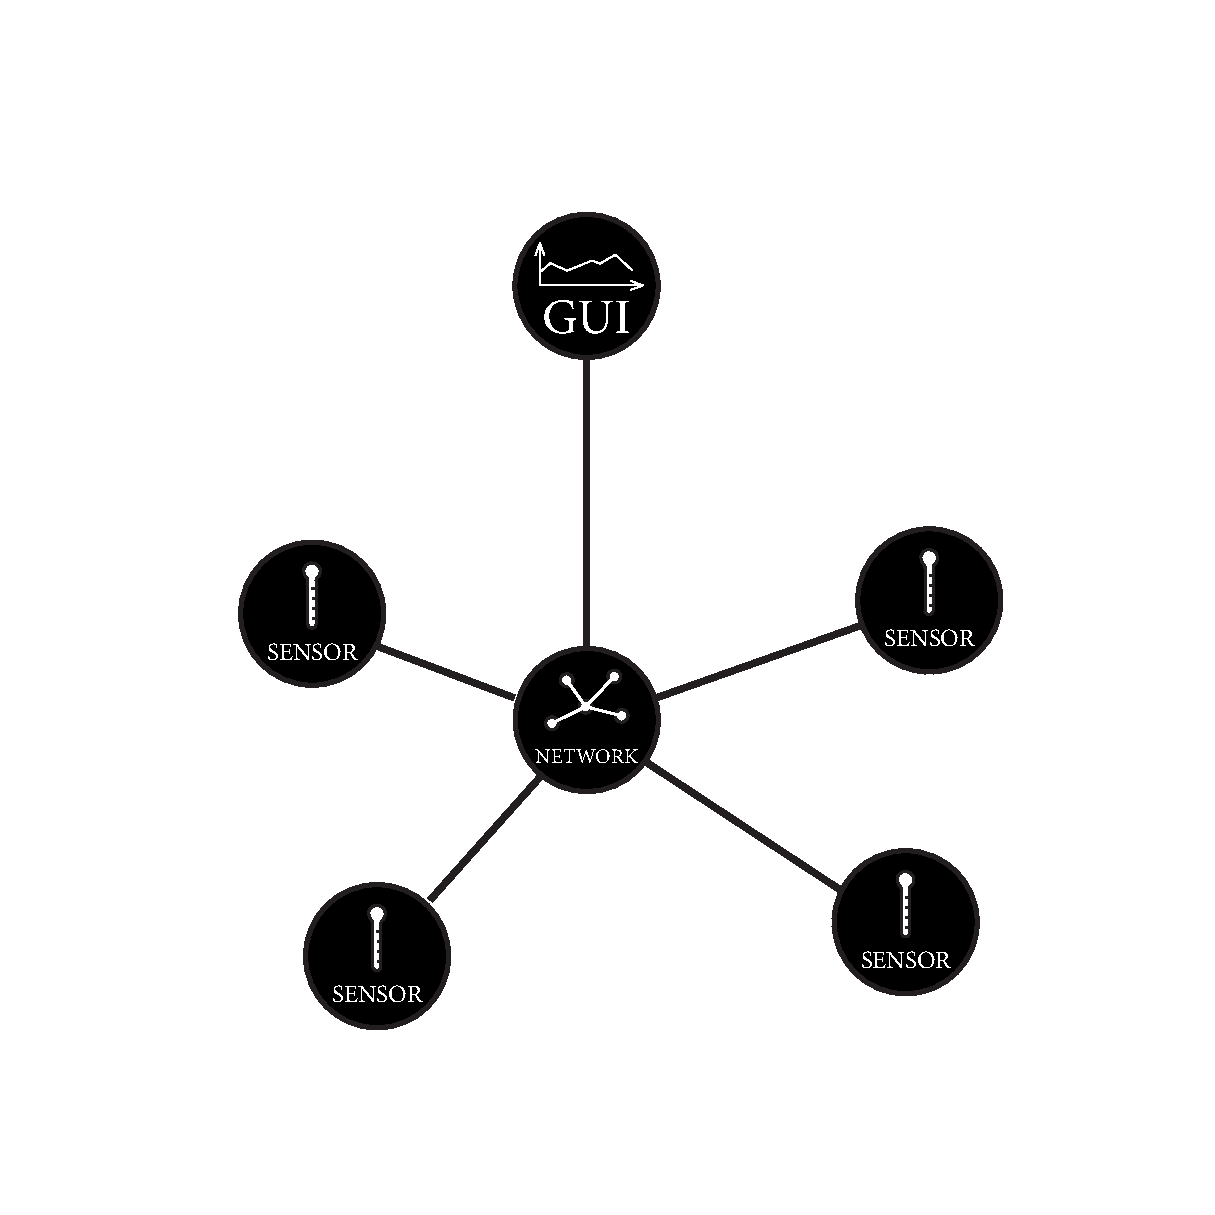
\includegraphics[width=.6\linewidth]{global_archi}
\caption[General Architecture]{\label{f:global_archi}General architecture.}
\end{figure}

To begin with, wireless communication protocols are explored. Once one is chosen and a hardware implementation is picked, we start exploring the system and show that drivers for peripherals can easily be written. Next, we continue with the interesting part of the system, the communications, and we finish by a method to share a common time among all nodes of the network.

All our work is available on our github : \url{https://github.com/Aunsiels/Mesh_Bee}

\section{Choosing a Wireless Protocol}
\label{s:Choosing a Wireless Protocol}

The first thing to think about is how to communicate. There are plenty of available protocols and we have to choose among them the one which will best fit to our needs. Eight protocols are considered: ZigBee, Bluetooth, BLE, Rubee, Zwave, ANT/ANT+, EnOcean and WiFi. To evaluate them, four characteristics are chosen: the data rate, the size, the consumption and the range. Of course, this properties depends of a lot of parameters : hardware, environment,... So, we try to choose values which appeared in most of the descriptions. The use cases are also useful to know what kind of things are possible with a protocol.

\subsection{The Protocols}
\subsubsection{Zigbee}

Zigbee is based on 802.15.4 specification, at 2.6 GHz. It is used in smart home, industrial control, medical tools, fire sensors... It is also used for low energy sensors, which is useful for us. A Ad Hoc network is created around a coordinator. Different architecture of the network are possible, we shall see it later. However, there can be problems with inferences as 2.4GHz is often used.

\subsubsection{Bluetooth}

Bluetooth is based on IEEE 802.15.1 and works at 2.6GHz. It is used in smart phones, keyboards, mice, sensors,... The fact that it is in all smart phone popularized in. The consumption is medium.

\subsubsection{BLE}

The Bluetooth Low Energy, just like Bluetooth, works at 2.4GHz. We can see it as a low consumption version of Bluetooth, which exists to answer modern problems like consumption. So, it is used in health care, sport, sensors...

\subsubsection{Rubee}

Rubee is a 450kHz protocol designed to transmit information in harsh environment (with a lot of steel for example), with high security. So, it is often used for military applications. It works with tags, a bit like NFC but the range can be higher. However, it is not that easy that find chip for Rubee development.

\subsubsection{Zwave}

Zwave is a protocol around 900MHz, designed for home automation applications. It can be integrated to a lot of existing of house products. It has a small consumption and a lower data rate than Zigbee.

\subsubsection{ANT/ANT+}

ANT/ANT+ works on 2.4GHz. It is a very low consumption protocol. It is mainly used in health, sport, smart home and industry.

\subsubsection{EnOcean}

EnOcean works on 902 MHz, 928.35 MHz, 868.3 MHz and 315 MHz and is a very low energy protocol (can also work without battery, inside a switch for example). The data rate is low. It can be used in smart house and in sensors.

\subsubsection{WiFi}

WiFi is a very popular protocol in personal application and is based on IEEE 802.11 . It operates on 2.4, 3.6, 5, and 60 GHz frequency bands. The speeds that can be achieve are high but the consumptions are also high. It is also used for the Internet of things and a lot of ship are now design with wifi integrated (Raspberry Pi 3, Arduino Genuino MKR1000, Red Pitaya, Electric Imp...).

\subsection{Comparing Protocols}

Everything is summarized in an odt file available on the github. The results are on sheet 1 and 2 and some results were plotted.

\begin{figure}[ht]
\centering
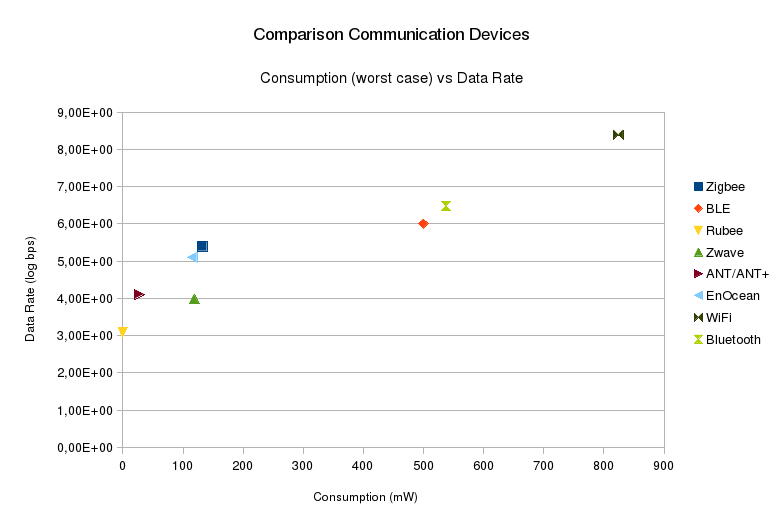
\includegraphics[width=.6\linewidth]{conso_vs_data_rate}
\caption[Consumption vs Data Rate]{\label{f:conso_vs_data_rate}Consumption vs Data Rate}
\end{figure}

We can see that each protocol is in a different area and so, we need to choose the one which will be good for us. For that, a cost function was design according to our needs. The function has four parameters (for the four protocol characteristics) that can be tuned. The chips available are also considered. Are they hard to get ? How easy is it to program them ? Is their help for it somewhere ? What are the prices ? Is it open sourced ? Finally we decide to go for Zigbee.

\subsection{Choosing a Zigbee Chip}

There are plenty of Zigbee chips available. What we want to find is a chip which controls both Zigbee and a sensor. So, the prototype can be programmed on the chip directly, without having to use an additional board like an Arduino. We also need to be able to read sensors thanks to I2C and ADC. There is a nice design, based on a NXP chip : the MeshBee. It is open source (both software and hardware) and easy to prototype with. Thus, thanks to it, we are able to first try to write a program to test if the prototype is working and then we will design a new chip in which sensors are directly integrated. That makes the final result smaller.

\section{Programming the Meshbee}

The embedded software on the MeshBee have to read data from a sensor and to send information through the network to the main node, the coordinator.

\subsection{Meshbee Framework}

First things first, we need to understand how MeshBee works.

\begin{figure}[ht]
\centering
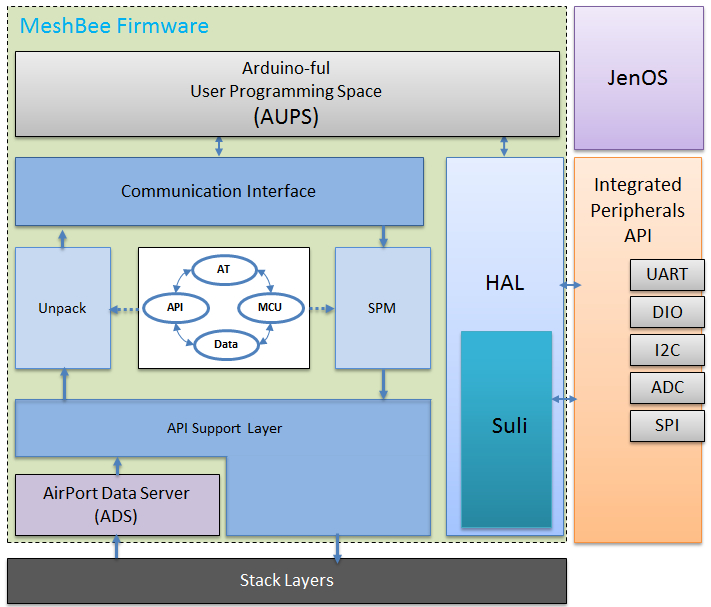
\includegraphics[width=.6\linewidth]{MeshBeeArchitecture}
\caption[MeshBee Architecture]{\label{f:MeshBeeArchitecture}MeshBee Architecture}
\end{figure}

The MeshBee firmware is built on an OS provided by NXP, JenOs, and a SDK for Low Energy Zigbee, also provided by NXP. It is important to know that because sometimes, the functions we are looking for (as interrupt-liked functions) are not in the MeshBee Framework but directly in the library provided by NXP.

Inside the MeshBee, we find an Arduino programming environment. The AUPS (Arduino-ful User Programming Space) provide two functions : a setup and a loop function. The setup function is called during the initialization of the system and the loop function is called periodically (it is possible to specify the period).

In the middle of Figure~\ref{f:MeshBeeArchitecture}, there are the four modes of the MeshBee :

\begin{itemize}
\item AT : this is an interactive mode. Easy commands have to be send to the MeshBee and it answers in an user-friendly way. To go to AT mode from everywhere, +++ have to be send.
\item API : this is a more effective and formatted way to communicate with the MCU. Thanks to it, AT function can be called from inside and outside the MCU, via UART for example. It is also possible send query to other nodes through the network thanks to the API commands.
\item MCU : this is the Arduino mode. The Arduino loop is only executed if the MeshBee is in this mode.
\item Data : this is a transparent mode : all data received on the Zigbee network are directly transmitted to UART and all data sent via UART are broadcast on the network.
\end{itemize}

The last thing to understand about this firmware is the Suli interface. This is a general library created by SeeedStudio. The goal is to make the interaction with GPIOs easier. So, for I2C, ADC,... there is no need to call the functions from JenOs but the easy functions provided by Suli can be used. However, we will need more advanced functions.

\subsection{Meshbee Hardware}

Figure~\ref{f:600px-Mesh_Bee_Pin} presents a picture of the hardware with the pin layout and Figure~\ref{f:pin_dispo} shows the pin layout in more details.

\begin{figure}[ht]
\centering
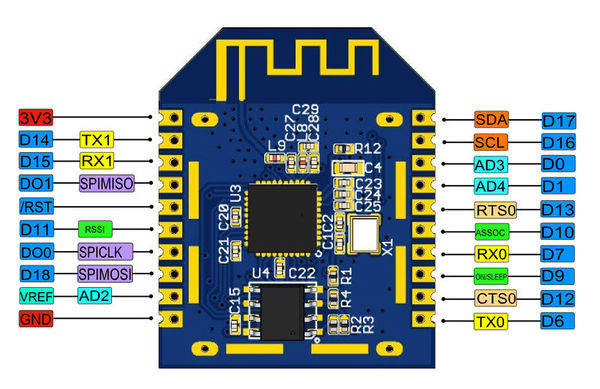
\includegraphics[width=.6\linewidth]{600px-Mesh_Bee_Pin}
\caption[MeshBee Hardware]{\label{f:600px-Mesh_Bee_Pin}MeshBee Hardware}
\end{figure}

\begin{figure}[ht]
\centering
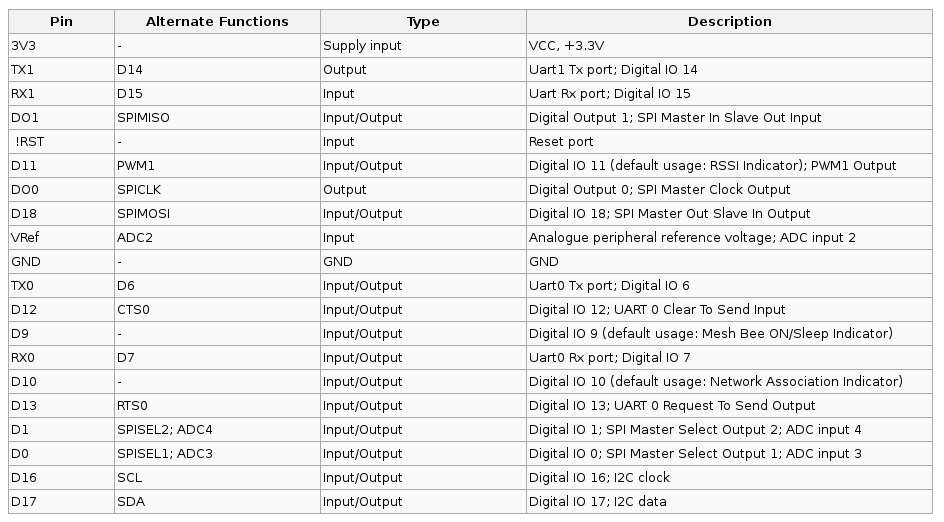
\includegraphics[width=.6\linewidth]{pin_dispo}
\caption[MeshBee Pin Layout]{\label{f:pin_dispo}MeshBee Pin Layout}
\end{figure}

\subsection{Tools}

NXP provides tools to program the Meshbee. These tools include a programmer and libraries to code the JN516X. More details about the installation are provided on our github : \url{https://github.com/Aunsiels/Mesh_Bee/blob/master/doc/documentation.md}.

\subsection{AT mode}

We have everything to compile so we are ready to communicate with the MeshBee. This communication uses \textbf{UART1}, so any USB-to-TTL working at \textbf{3.3V} (this is very important) device would work. For now, we only use the official programmer. We just switch the left switch to UART1 (up). Then, a serial communication tool is used to communicate. The Baud is \textbf{115200}, there is \textbf{no parity bit}, \textbf{8 data bits}, \textbf{1 stop bit} and \textbf{no flow control}.

When we send an AT command, it is important to have \textbf{CR} (which is \r) at the end of the line. It will not be specify in the rest of the text.

It is time for our first command : \textbf{+++}. This allows us to go to AT mode. We receive an \textbf{Enter AT Mode} if we were not in AT mode yet or an \textbf{Error, invalid command} if we were in AT mode.

AT commands are composed as follow : \textbf{ATXX[YYYY]}. They always begin by AT. Then follow two characters to identify the command, for example IF or AJ. Then follow up to 4 optional numbers which are parameters of the command. For more about it, everything was explained in details in the AT commands section in the User's Manual. We note by looking at the code (that's something we have to often do) that all commands are not available for all device type. For instance, an end-node is not able to create a network and thus do not have this command.

Here is a list of useful commands. We begin with \textbf{ATIF}. This prints information about the MeshBee. We check that the Device Type is the one we think, the coordinator for example. With the coordinator, we send \textbf{ATPA1}. This command creates a new network. The MeshBee is reset and the ASSOC led on the programmer light up. We send \textbf{ATIF} again and read the \textbf{PANID} field, which is the id of our network. We can go to an other mode, for example data mode with \textbf{ATDT}.

\begin{figure}[ht]
\centering
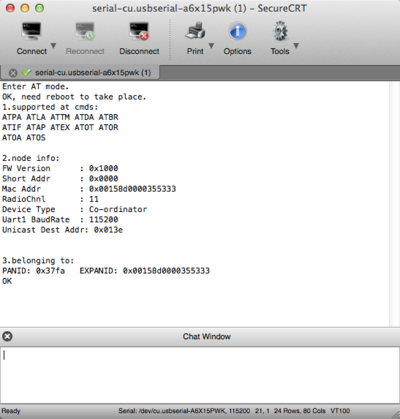
\includegraphics[width=.6\linewidth]{400px-Configure_coo2}
\caption[Result ATIF]{\label{f:400px-Configure_coo2}Result ATIF}
\end{figure}

Next, an other node is connected to the network. We have to remember that we always need the coordinator to be on. We unplug it from the programmer and give it power with the raspberry pi (see below). We want to be sure that it is connected, so a LED is also connected (and a resistor !) to the ASSOC pin (We were able to read the names of the pins below the MeshBee but there is also Figure~\ref{f:600px-Mesh_Bee_Pin} above to check). A node is plugged in the programmer. It had been flashed with the router or end-node code.

As before, we go to AT mode with +++ and get information with ATIF. If the MeshBee was not configured before, the PANID is 0x0000 or a number different from the one of the coordinator. We have to say to our device to automatically join a network with \textbf{ATAJ1}. Then the network is rescanned with \textbf{ATRS} and after some seconds, the ASSOC led light up. We check information with ATIF and then we have the same PANID than the coordinator. To know what are the other nodes on the network, we send the \textbf{ATLA} command. That sends a request to all nodes and we receive information about all of them. We go to data mode with \textbf{ATDT} and everything which is typed in the console is broadcast on the network. As the coordinator is also linked to a serial port, the raspberry pi one (see below), we see that our messages appear in the coordinator console.


\subsection{MCU mode}

The MCU mode is the "Arduino like" mode. We go to this mode from the AT mode by just typing \textbf{ATMC}. Then, the Arduino-loop start.

\subsubsection{The Arduino-like functions}

The source code is located in \textbf{src}, on the github. One of the file is called ups\_arduino\_sketch.c . This file contains the two Arduino-like functions : \textbf{arduino\_setup} and \textbf{arduino\_loop}.

The \textbf{arduino\_setup} function is called when entering in MCU mode, through the function ups\_init we find in firmware\_aups.c (AUPS stands for Arduino User Programming Space). This function also calls suli\_init, so there is no need to initialize Suli (see below) if the device is in MCU mode. In the arduino\_setup function, everything that needs to be done at the beginning of our program is written, for example initialization of peripherals.

The \textbf{arduino\_loop} was a function which was called periodically. We define the time between two loops by typing in AT mode, \textbf{ATMFXXXX} where XXXX is a number between 0 and 3000 and is the time in milliseconds between two Arduino\_Loop. This Arduino\_Loop function is a task, defined in firmware\_aups.c, and either calls arduino\_loop or exits MCU mode to AT mode if +++ is read.

We notice that here we have to use the C preprocessor to know for which device we are compiling the program for.

\begin{lstlisting}[frame=single]
#ifdef TARGET_COO
// Code for the coordinator
#elif TARGET_ROU
// Code for the router
#else
// Code for the end node
#endif
\end{lstlisting}

\subsection{The SULI Library}

SULI is a library written by SeeedStudio to easily use the peripherals. It is imported it by just adding :

\begin{lstlisting}[frame=single]
#include "suli.h"
\end{lstlisting}

When the device is in MCU mode, we do not need to initialize Suli. Otherwise :

\begin{lstlisting}[frame=single]
suli_init();
\end{lstlisting}

\subsubsection{Simple GPIO}

Our first experiment is with simple input/output. First, we need to initialize the pin. We need to use the \textbf{void suli\_pin\_init(IO\_T *pio, PIN\_T pin}) function. It takes two arguments : an IO\_T variable that contains the properties of the pin and the pin number.

\begin{lstlisting}[frame=single]
IO_T led_io;
suli_pin_init(&led_io, D9);
\end{lstlisting}

The pin number is either an int or a defined pin name (they are defined in suli/suli.h) :

\begin{lstlisting}[frame=single]
D0 = 0, D1=1, D2, D3, D4, D5, D6, D7, D8, D9, D10, D11,
D12, D13, D14, D15, D16, D17, D18, D19, D20, DO0=33,
DO1=34, A3=0, A4=1, A2=50, A1, TEMP, VOL
\end{lstlisting}

Then we have to set the direction, input or output, of the pin. We use the \textbf{void suli\_pin\_dir(IO\_T *pio, DIR\_T dir)} function, which takes a IO\_T argument and a direction, which could either be \textbf{HAL\_PIN\_OUTPUT} or \textbf{HAL\_PIN\_INPUT}.

The state of a pin can be read with \textbf{int16 suli\_pin\_read(IO\_T *pio)} and be written with \textbf{void suli\_pin\_write(IO\_T *pio, int16 state)}. The state can either be \textbf{HAL\_PIN\_HIGH} or \textbf{HAL\_PIN\_LOW}.

A pulse could be read with \textbf{uint32 suli\_pulse\_in(IO\_T *pio, uint8 state, uint32 timeout)}, which returns the length of the pulse in microseconds.

\subsubsection{ADC}

Like for simple input/output, the pin need to be initialized for analog reading first. We use \textbf{void suli\_analog\_init(ANALOG\_T * aio, PIN\_T pin)} where ANALOG\_T was the equivalent of IO\_T. For the pin, there is a choice between A3=0, A4=1, A2=50, A1, TEMP, VOL. Then, we are able to read with\textbf{ int16 suli\_analog\_read(ANALOG\_T *aio)}.

\begin{lstlisting}[frame=single]
ANALOG_T temp_pin;
suli_analog_init(&temp_pin, TEMP);
int16 temper = suli_analog_read(&temp_pin);
\end{lstlisting}

\subsubsection{Time functions}

We find two functions in Suli to wait a certain amount of time : \textbf{void suli\_delay\_us(uint32 us);} for microseconds waiting and \textbf{void suli\_delay\_ms(uint32 ms);} for milliseconds waiting. We also find a function to know for how long the program have been running : \textbf{uint32 suli\_millis(void);} for milliseconds and \textbf{uint32 suli\_micros(void);} for microseconds. There could be overflow, after 50 days for suli\_millis but after 70 minutes for suli\_micros.

Because of these overflows, the time functions are modified to return an uint64. This will be important for time synchronization.

\subsubsection{I2C}

I2C works the same way than ADC and input/output. There is an initialization function \textbf{void suli\_i2c\_init(void * i2c\_device);}, a write function \textbf{uint8 suli\_i2c\_write(void * i2c\_device, uint8 dev\_addr, uint8 *data, uint8 len);} and a read function \textbf{uint8 suli\_i2c\_read(void * i2c\_device, uint8 dev\_addr, uint8 *buff, uint8 len);}. For I2C, as we had no choice for the pin, specify the i2c\_device is useless. We just gave NULL.

\begin{lstlisting}[frame=single]
suli_i2c_init(NULL);
uint8 data = TRIGGER_HUMD_MEASURE_NOHOLD;
suli_i2c_write(NULL, HTDU21D_ADDRESS, &data, 1);
uint8 msb;
suli_i2c_read(NULL, HTDU21D_ADDRESS, &msb, 1);
\end{lstlisting}

We write a use example of I2C in \textbf{src/humidity.c}. This is a driver to read data from a humidity and temperature sensor (see below).

\subsubsection{UART}

Like I2C, we have no choice for the UART Port, it has to be UART1. So, in the initialization function \textbf{void suli\_uart\_init(void * uart\_device, int16 uart\_num, uint32 baud);}, there is no need to specify uart\_device and uart\_num. The baud can be : 4800, 9600, 19200, 38400, 57600 or 115200. We notice that by default, the baud rate is initialized to 115200, so there is no special need to initialize it.

For the writing part, there is a general function, \textbf{void suli\_uart\_send(void * uart\_device, int16 uart\_num, uint8 *data, uint16 len);} which just takes an array of data and the length of this array. Then, there are more specific functions : \textbf{void suli\_uart\_send\_byte(void * uart\_device, int16 uart\_num, uint8 data);}, \textbf{void suli\_uart\_write\_float(void uart\_device, int16 uart\_num, float data, uint8 prec);}, \textbf{void suli\_uart\_write\_int(void * uart\_device, int16 uart\_num, int32 num);}. However, we want to use printf-like function, much easier to use. So, most of the time, we used \textbf{void suli\_uart\_printf(void uart\_device, int16 uart\_num, const char *fmt, ...);} (the three dots are a notation of C to say that the number of argument is undetermined, as it is in printf). This function does not work well for float.

\begin{lstlisting}[frame=single]
suli_uart_printf(NULL, NULL, "<HeartBeat%d>\r\n",
                 random());
\end{lstlisting}

For the reading part, we have a function to know if there is something to read : \textbf{uint16 suli\_uart\_readable(void *uart\_device, int16 uart\_num);} which returns one if UART has received readable data, zero otherwise. Then we are able to read a byte with \textbf{uint8 suli\_uart\_read\_byte(void *uart\_device, int16 uart\_num);}

\subsection{API MODE}

The API is a simple way to communicate with the MCU from outside. The messages have a particular form, which is explained in details in the User's Manual. It is also possible to call API commands from MCU mode.

\subsubsection{API Frames}

The API frame must have a specific form, which depends on what we want to do. The frames are described in the User's Manual.

\subsubsection{Send API Commands from MCU Mode}

To send an API Command, we need to build a tsApiSpec, which is a representation of an API Frame. Here is what is inside :

\begin{lstlisting}[frame=single]
/* API-specific structure */                                                                             
typedef struct                                                                                           
{                                                                                                        
    uint8 startDelimiter;   
    // start delimiter '0x7e'                                                    
    uint8 length;           
    // length = sizeof(payload)                                                  
    uint8 teApiIdentifier;  
    //indicate what type of packets this is                                      
    union                                                                                                
    {                                                                                                    
        /*diff app frame*/                                                                               
        uint8 dummyByte;            
        //dummy byte for non-information frame                               
        tsNwkTopoReq nwkTopoReq;                                                                         
        tsNwkTopoResp nwkTopoResp;                                                                       
        tsLocalAtReq localAtReq;                                                                         
        tsLocalAtResp localAtResp;                                                                       
        tsRemoteAtReq remoteAtReq;                                                                       
        tsRemoteAtResp remoteAtResp;                                                                     
        tsTxDataPacket txDataPacket;                                                                     
        tsOtaNotice    otaNotice;    
        //OTA notice message                                                
        tsOtaReq otaReq;                                                                                 
        tsOtaResp otaResp;                                                                               
        tsOtaStatusResp otaStatusResp;                                                                   
    }__attribute__ ((packed)) payload;                                                                   
    uint8 checkSum;      //verify byte                                            
}__attribute__ ((packed)) tsApiSpec;
\end{lstlisting}

We do not care about startDelimiter, it was always 0x7e and is set for us by a function. Then come the length of the payload, which is the useful data in the frame. The teApiIdentifier is the id to identify a packet. It can be one of the following option :

\begin{lstlisting}[frame=single]
typedef enum
{
    /* API identifier */
    API_LOCAL_AT_REQ = 0x08,      
    //local At require
    API_LOCAL_AT_RESP = 0x88,    
    //local At response
    API_REMOTE_AT_REQ = 0x17,    
    //remote At require
    API_REMOTE_AT_RESP = 0x97,   
    //remote At response
    API_DATA_PACKET = 0x02,      
    //indicate that's a data 
    //packet,data packet is certainly remote packet.
    API_TEST = 0x8f,             
    //Test
    API_OTA_NTC = 0xd3,
    API_OTA_REQ = 0xb0,
    API_OTA_RESP = 0x06,
    API_OTA_ABT_REQ = 0xf7,
    API_OTA_ABT_RESP = 0xdb,
    API_OTA_UPG_REQ = 0x5a,
    API_OTA_UPG_RESP = 0xe6,
    API_OTA_ST_REQ = 0x91,
    API_OTA_ST_RESP = 0x89,
    API_TOPO_REQ = 0xfb,
    API_TOPO_RESP = 0x6b
}teApiIdentifier;
\end{lstlisting}

Depending of what we are sending, we have to choose the correct id. They are described in the User's Manual. Then, there is a union, payload. In C, it simply means that we have to choose one of the following options. The \_\_attribute\_\_((packed)) means that the compiler has to put all the fields together, without a hole, in the memory : they are "packed"". We notice that in the payload, we have for example localAtReq to make, as the name said, a local At request. To find the exact definition of a payload, we go to \textbf{include/firmware\_at\_api.h}. Then, finally, we have a checksum which helps us to be a more sure that data are transmitted without problems (like a bit switch).

Most of the time, we do not have to complete the tsApiSpec ourself. Functions are provided to make it easier. It is also the case for tsLocalAtResp and tsRemoteAtResp.

For example, if we want to send data to another node in the network. It could be done by sending a API command.

\begin{lstlisting}[frame=single]
#include "firmware_at_api.h"
#include "firmware_api_pack"
//Those two include contains the function
//to easily create tsApiSpec and send them

tsApiSpec apiSpec;
uint8 tmp[sizeof(tsApiSpec)]={0}; 
// Will contain the final result
//For now we put in it a string
sprintf(tmp, "TEST %d", 3); 
// Just a formatted string (like in printf) in tmp
PCK_vApiSpecDataFrame(&apiSpec, 0xec,
                      0x00, tmp, strlen(tmp));
// This function create a DataFrame
uint16 size = i32CopyApiSpec(&apiSpec, tmp); 
//We actually create the array containing 
//the API Frame in tmp
API_bSendToAirPort(UNICAST, 0x0000, tmp, size);
// We send the message to 0x0000, the coordinator
\end{lstlisting}

To fill tsApiSpec, we use, for data, \textbf{void PCK\_vApiSpecDataFrame(tsApiSpec *apiSpec, uint8 frameId, uint8 option, void *data, int len);} in firmware\_api\_pack.h. The frameId just identified the frame, we put whatever we want, it is not that important. The option is 0 for UNICAST, 1 for BROADCAST. It is also important to create the actual frame inside an array with \textbf{int i32CopyApiSpec(tsApiSpec *spec, uint8 *dst);} also in firmware\_api\_pack.h. It returns the size of the frame, which is useful when we want to send my frame with \textbf{bool API\_bSendToAirPort(uint16 txMode, uint16 unicastDest, uint8 *buf, int len);} in firmware\_at\_api.h. The txMode can be either UNICAST (to only one node) or BROADCAST (to all nodes). Then we have to specify an address which is only used if we are in UNICAST mode (otherwise it does not matter), the frame array we have just created and its length.

We are also able to call AT commands thanks to \textbf{int API\_i32AtCmdProc(uint8 *buf, int len);} in firmware\_at\_api.h. We just give it a command and its length and it returns if the function has succeeded or not.

\begin{lstlisting}[frame=single]
char * aj = "ATAJ1";
API_i32AtCmdProc(aj, 5);
\end{lstlisting}

We find other functions in firmware\_at\_api.h and firmware\_api\_pack.h but for now we do not find them useful. It is for example possible to send a message to a given Mac address. We explore the code if we want to go in more details.

\subsection{Create New Tasks}

Sometimes, we may need to call a given function every one second. In JenOs, we need to create a new \textbf{Task}. Tasks are special functions which can only be called by the OS. They are run in parallel of the main function (so we need to be careful with shared resources). The first thing we have to do is to say to the OS to add a new task. This is done in the file \textbf{src/MeshBee.oscfgdiag}. When we open the raw files, there is a lot of text and it is hard to understand everything. NXP provides a graphical interface to edit this file. We use it.

In the Jennic/Tools, we can find eclipse, a well-known code editor. The file is still a raw text when we open it. We have to choose plugins in Jennic/Tools/Eclipse\_plugins. Once the plugins are installed, the raw text becomes a diagram.

\begin{figure}[ht]
\centering
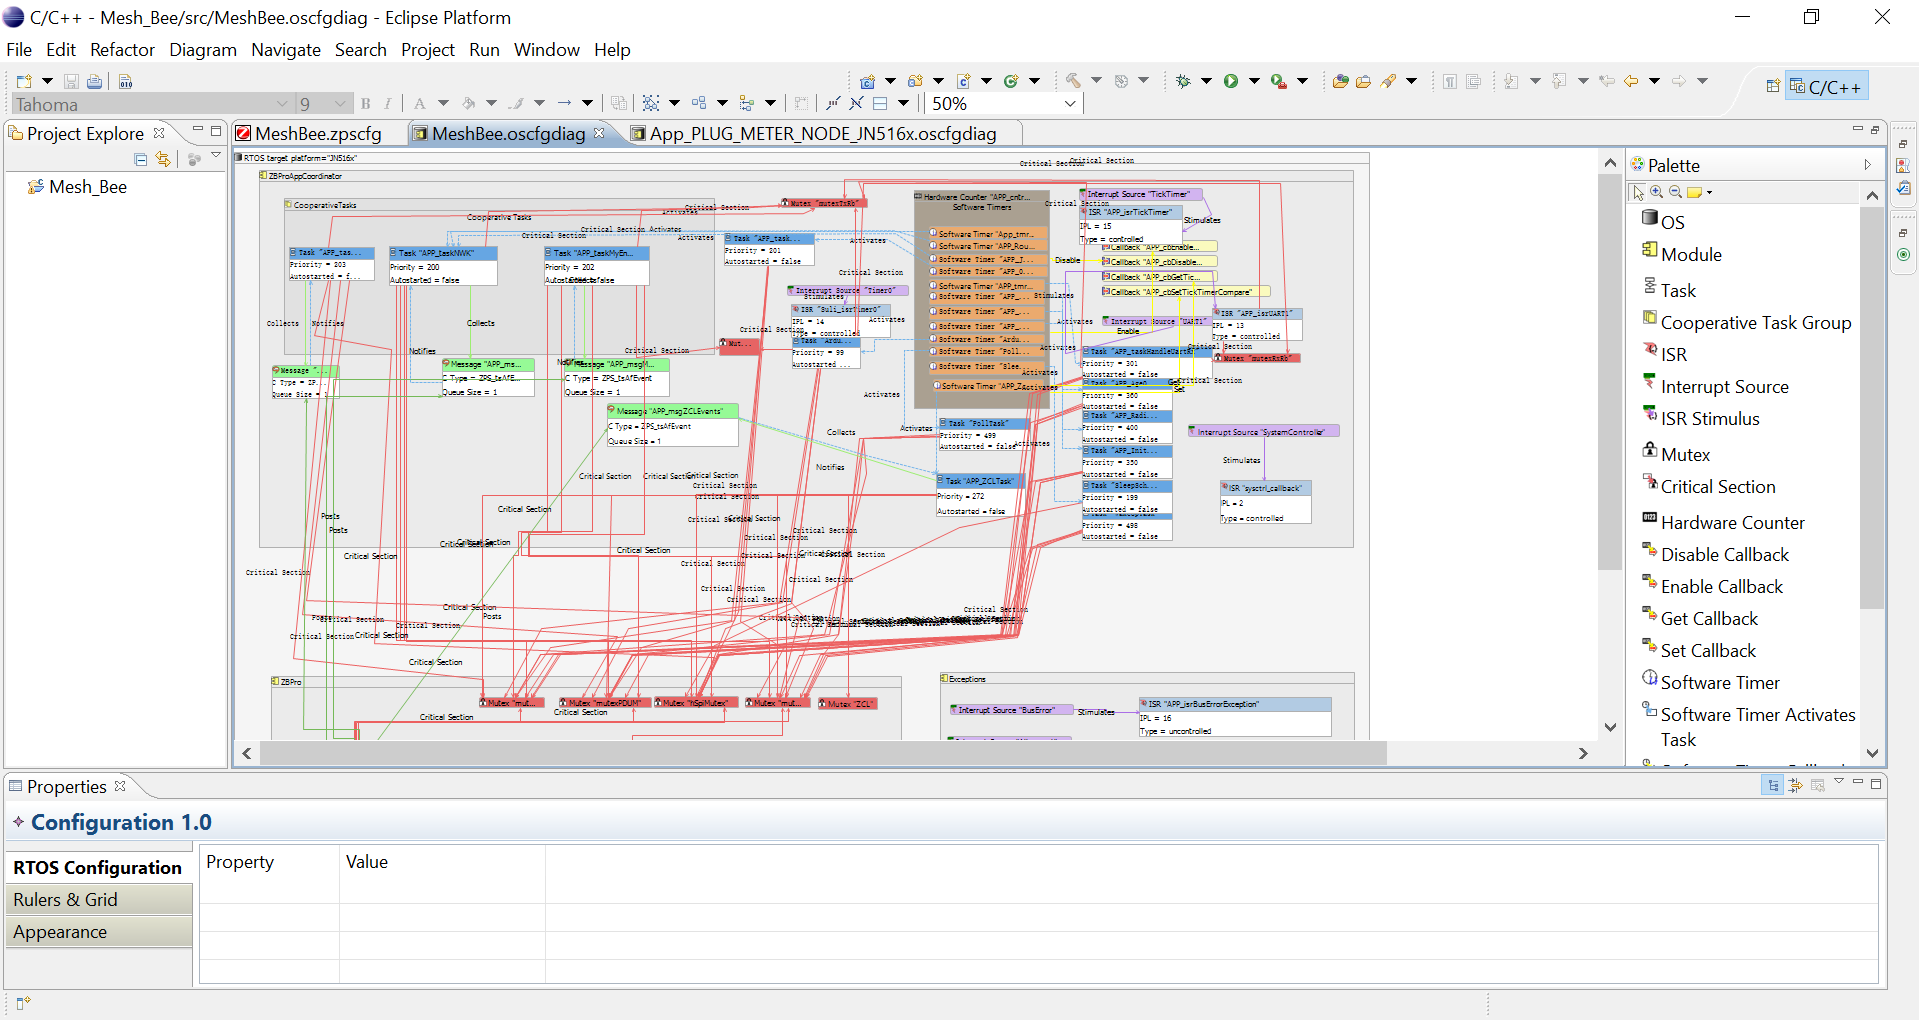
\includegraphics[width=.6\linewidth]{eclipse}
\caption[Eclipse Configuration file]{\label{f:eclipse}Eclipse configuration file}
\end{figure}

We see, on the left, the project explorer where are our files. On the right, there are the components that can be added in the diagram, which is in the middle if it was opened. At the bottom, there are the properties of the selected component. If it is not there, it can be added by clicking on the bottom left hand corner icon and by selecting "Properties".

We look at diagram in more details.

\begin{figure}[ht]
\centering
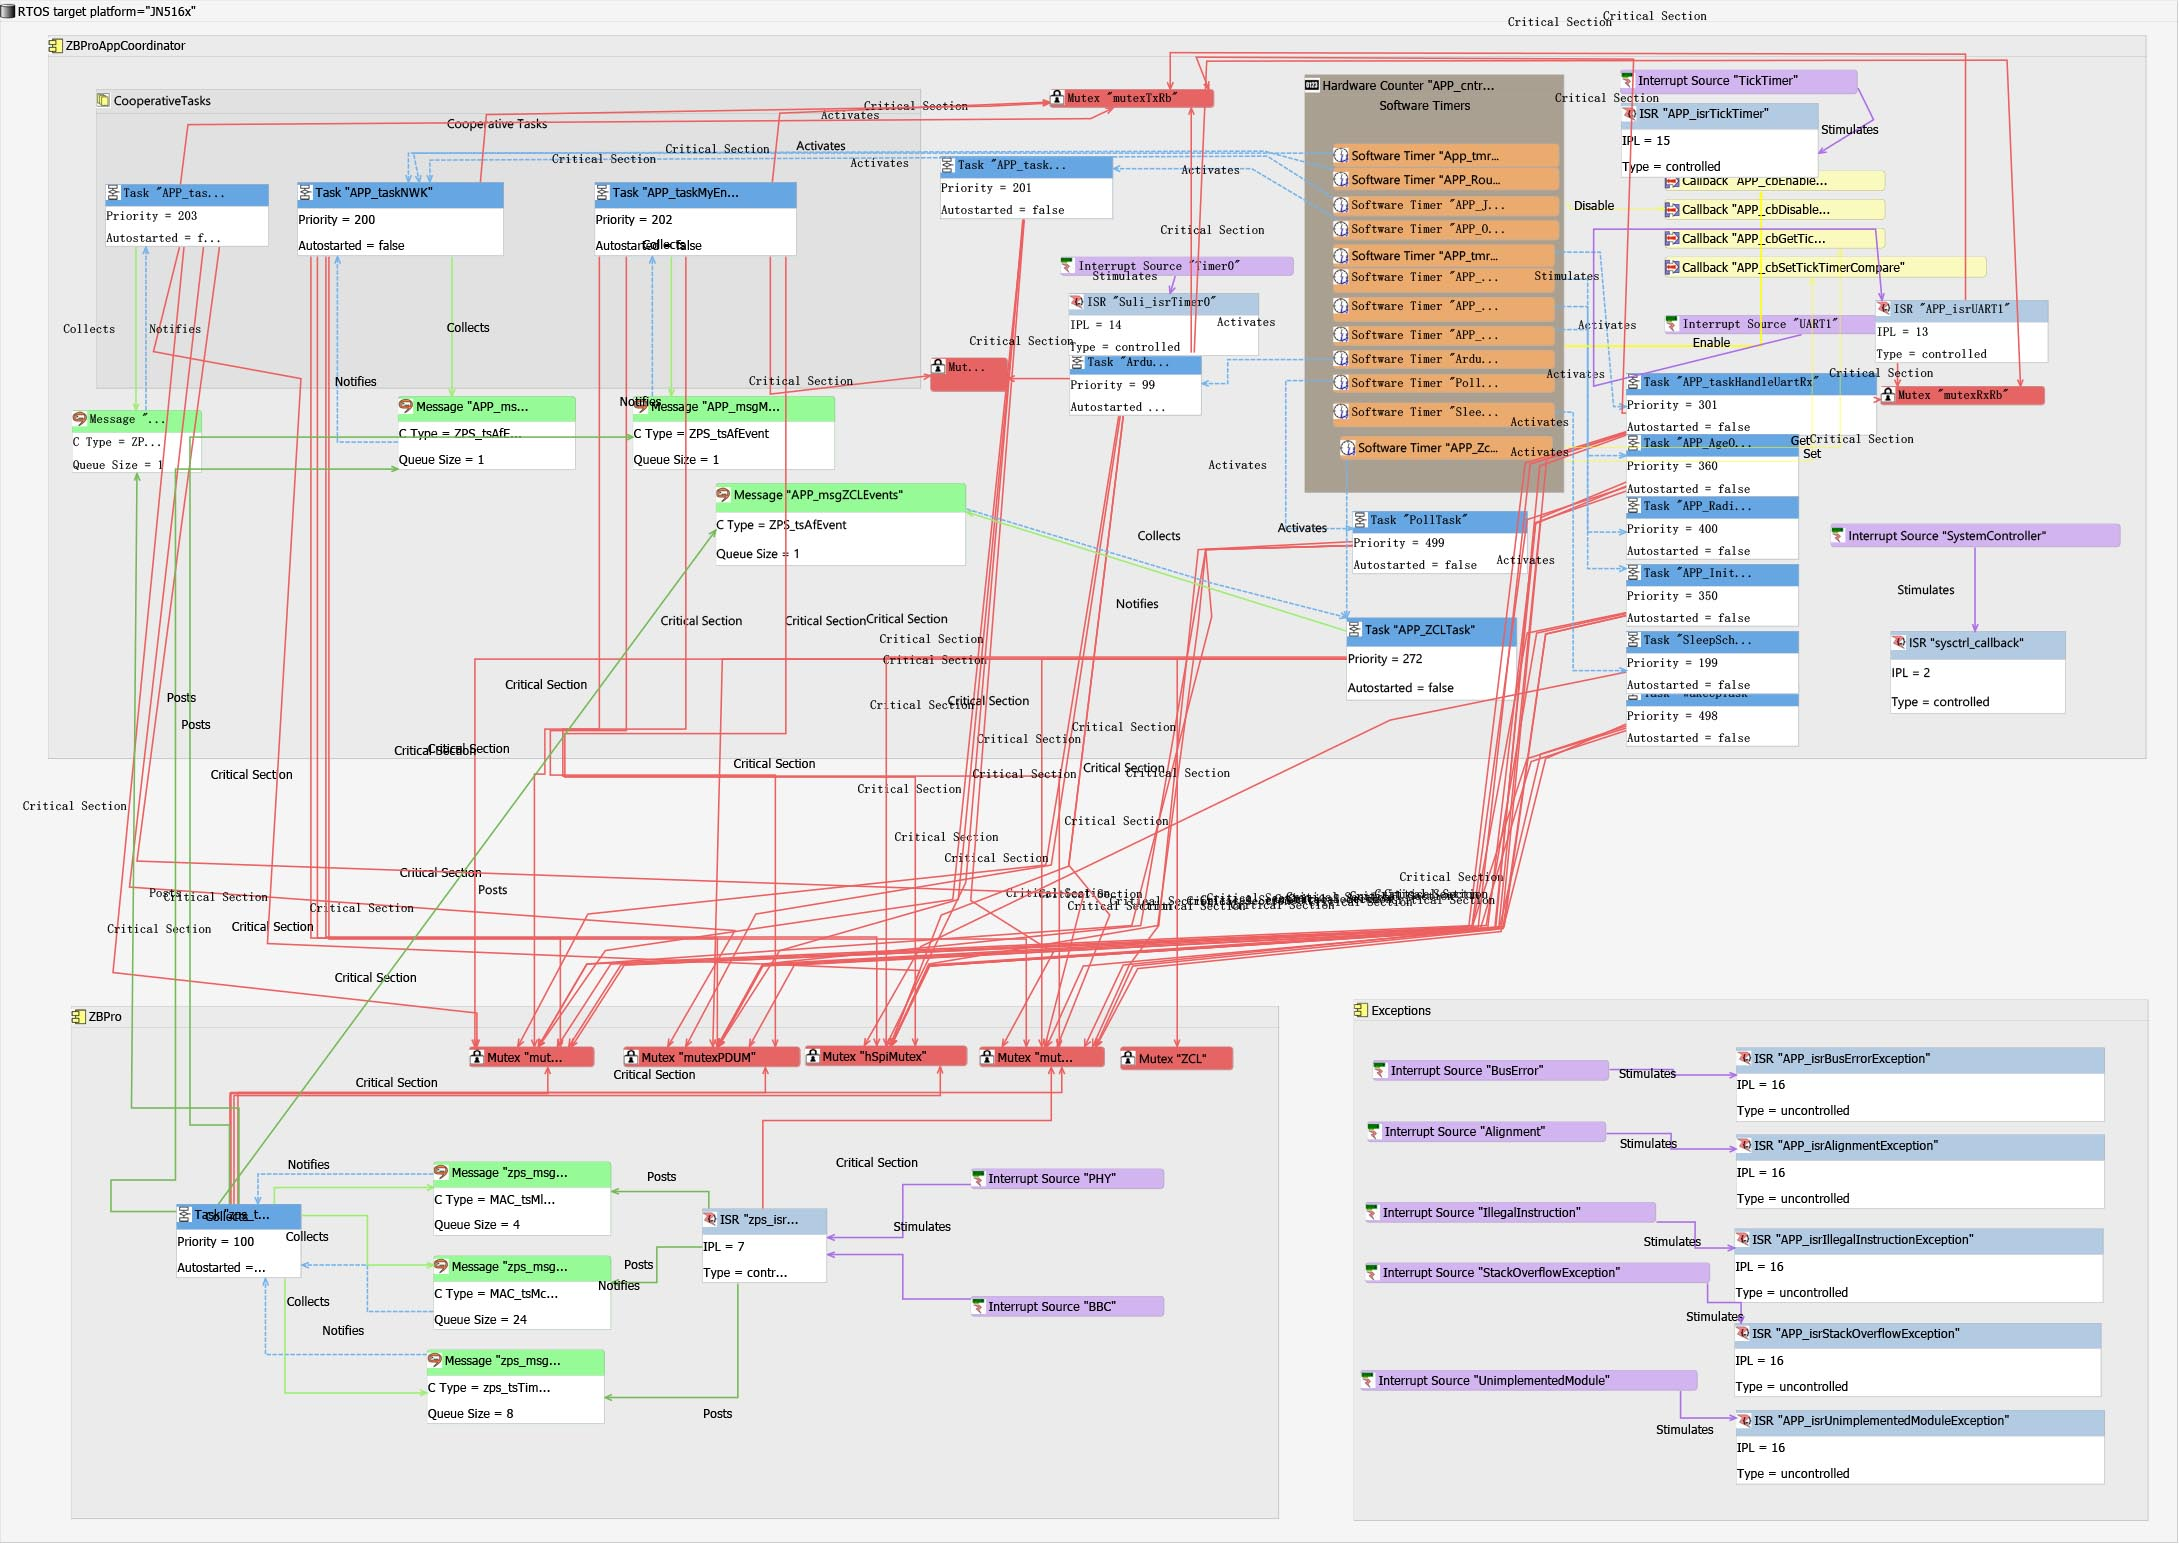
\includegraphics[width=.6\linewidth]{global_config}
\caption[Details Configuration]{\label{f:global_config}Details configuration}
\end{figure}

We can see that there are different kinds of blocks : Tasks, Software Timer, mutexes... These blocks are linked to each other in a meaningful way. For instance, a task is able to use a mutex to enter in a critical section. We notice that sometimes the documentation of JenOs assumes that some blocks are declared. For example, it is assumed that there is a task declared for time synchronization or that there is an interrupt handler for System Controller's interrupts. So, the first time we discovered it, it was a bit surprising that given function do not work. If it was written to give a callback function for an interrupt, even if the function existed, if there was nothing in the configuration file to declare the interrupt and link it to an ISR (see later to know what it is), the function was useless and did not work at all.

We create a task to synchronize time. The task name was APP\_ZCLTask. The goal of the task is to keep the count of the time (see later). We just select Task in the Palette. Then, we click in a free space in the diagram. The Task box appears. We give it a name and a priority (for the scheduler). Then are created links with other components. Some links can be created directly by using the input and output arrows at the border of the box (they appear when passing the mouse above the box). Some links need to be selected in the Palette. It is the case for Critical Section.

\begin{figure}[ht]
\centering
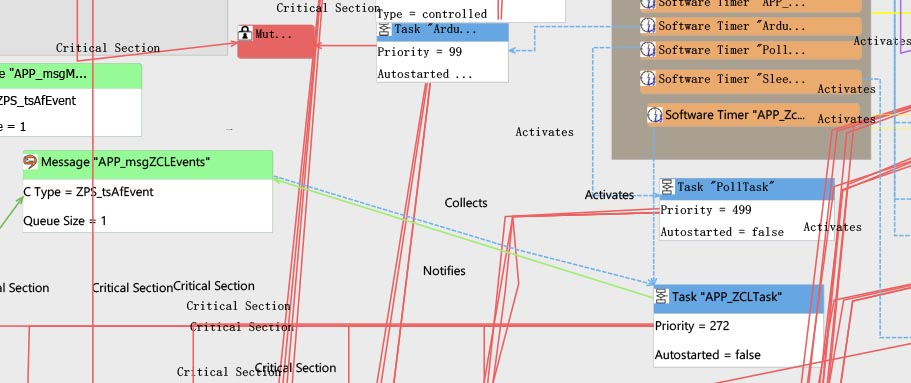
\includegraphics[width=.6\linewidth]{zoom_softtimer}
\caption[Zoom configuration]{\label{f:zoom_softtimer}Zoom configuration}
\end{figure}

The task is declared to the OS. A file will be generated at compile time to transform those information into code. The files generated are called build/gen/os\*.

We then have to add code to explain to the OS what to do with the task. To declare the task, we use the macro : \textbf{OS\_TASK(task\_name)}. For example, if the task's name was App\_Task, it looks like :

\begin{lstlisting}[frame=single]
OS(APP_Task) {
    // Code
}
\end{lstlisting}

The task is created. We need to say when to execute our task. The easiest way to it is to use the function \textbf{OS\_teStatus OS\_eActivateTask(OS\_thTask hTask);}. It takes the task name as an argument and returns if it succeeded or not : OS\_E\_OK (successful), OS\_E\_BADTASK (invalid task handle used) or OS\_E\_OVERACTIVATION (maximum number of activations exceeded: 65535). It asks the OS to schedule the given task. However, it is quite limited because we need to know exactly when to call the task. However, we need to call the task every second. So, we need to use a timer, the one we declared in our configuration file. We have a function to say to start the timer : \textbf{OS\_teStatus OS\_eStartSWTimer(OS\_thSWTimer hSWTimer, uint32 u32Ticks, void *pvData);}. It takes the timer's name, the number of ticks before the timer ends (we used the macro \textbf{APP\_TIME\_MS(n\_milliseconds))}, and data which are only useful for callback functions (here we provided NULL for our task). It returns a status which could be OS\_E\_OK (successful), OS\_E\_BADSWTIMER (invalid software timer handle) or OS\_E\_SWTIMER\_RUNNING (software timer already running). Once our task is called, it is either possible to restart the timer with the same function or to continue to use the same timer (which continues to count while we do some computation) with \textbf{OS\_teStatus OS\_eContinueSWTimer(OS\_thSWTimer hSWTimer, uint32 u32Ticks, void *pvData);} (returns the same status than OS\_eStartSWTimer). Finally, we need to check the status of the timer with \textbf{OS\_teStatus OS\_eGetSWTimerStatus(OS\_thSWTimer hSWTimer);} to know whether it has just expired or not. It returns either OS\_E\_BADSWTIMER (invalid software timer handle), OS\_E\_SWTIMER\_RUNNING (software timer is running), OS\_E\_SWTIMER\_STOPPED (software timer has been stopped) or OS\_E\_SWTIMER\_EXPIRED (software timer has expired).

For applications, see later, in time synchronization v1 for example.

\subsection{Interrupt From a Button}

To try our time synchronization, we need a physical common event. Our first experiment is carried out with a simple button. Later, it will be replaced by an interrupt from a sensor for example, to trigger a measurement for instance. An interrupt is something which has to be scheduled by the OS, so we need to declare it in the configuration file. The document claims that they have a function a register a callback for I/O interrupts but it does not work. So, we declare an interrupt source, System Controller. System controller gathered different kind of interrupt among which the IO ones. Then we declare a task, sysctrl\_callback, which was stimulated by the interrupt source we have just created.

\begin{figure}[ht]
\centering
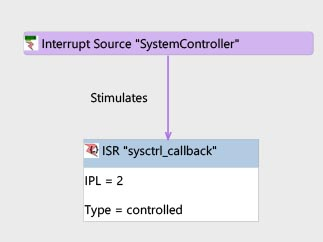
\includegraphics[width=.6\linewidth]{zoom_interrupt}
\caption[Zoom Interrupt]{\label{f:zoom_interrupt}Zoom Interrupt}
\end{figure}

The interrupt function is defined in \textbf{src/utils\_meshbee.c}. It sends a simple frame to the server when the button is pressed. The button is initialized in the arduino\_setup function. Suli was not enough so we have to use functions from JenOs :


\begin{lstlisting}[frame=single]
uint32 mask = (1 << D0);
vAHI_DioSetDirection(mask, 0);
vAHI_DioInterruptEdge(0, mask);
// First argument for rising edge
vAHI_DioInterruptEnable(mask, 0);
\end{lstlisting}

The mask simply indicats which IOs are concerned by a change. We need to set to 1 the bit at the position of the number of the IO. \textbf{vAHI\_DioSetDirection} set the direction of the pin, the first arguments are the pins we want to change to input and the second to output. \textbf{vAHI\_DioInterruptEdge} allowed us to change the edge which triggers the interrupt, the first argument being falling and the second rising. Then \textbf{vAHI\_DioInterruptEnable} was used to enable the interrupt (first argument) or to disable it (second argument).

\section{Examples}

The first experiments we carry out allow us to better understand how it works. We begin with a simple hello word, with a LED. We will continue with more complex peripherals.

\subsection{Hello World !}

The circuit is really simple : a Led and a resistor connected to D9.

\begin{figure}[ht]
\centering
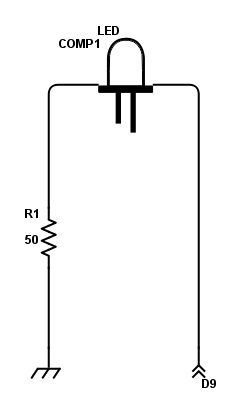
\includegraphics[width=.6\linewidth]{led_scheme}
\caption[Simple Led]{\label{f:led_scheme}Simple Led}
\end{figure}

The code we use is also simple.

\begin{lstlisting}[frame=single]
#include "suli.h"

IO_T led_io;
int state;

void arduino_setup(void){
    suli_pin_init(&led_io, D9);
    suli_pin_dir(&led_io, HAL_PIN_OUTPUT);
    state = HAL_PIN_OUTPUT; 
    // contains the current state of the LED
    suli_pin_write(&led_io, state);
}

void arduino_loop(void){
    state = ~state; 
    // We just exchange the state of the pin

    suli_pin_write(&led_io, state); //Blink

    suli_delay_ms(1000); // wait one second
}
\end{lstlisting}

Note that instead of waiting actively with suli\_delay\_ms, we could also change the period of the arduino loop with ATMF1000.

\subsection{Read a Brightness}

To measure the brightness, we use a photo-resistor : the higher the brightness the lower the resistance. So, to measure it, we do a voltage divider with a resistor of 5K ohms.

\begin{figure}[ht]
\centering
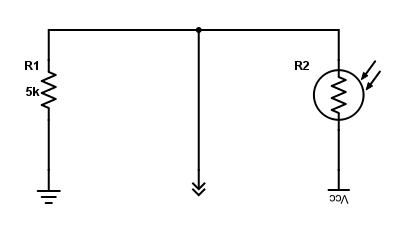
\includegraphics[width=.6\linewidth]{photores}
\caption[Photoresistor]{\label{f:photores}Photoresistor}
\end{figure}

We connect the middle point with ADC3, i.e. D0. Here is the code, we read the brightness and send it to the coordinator :

\begin{lstlisting}[frame=single]
#include "suli.h"
#include "firmware_api_pack.h"
#include "firmware_at_api.h"

ANALOG_T brightness_pin;

void arduino_setup(void){
    suli_analog_init(&brightness_pin);
}

void arduino_loop(void){
    uint8 tmp[sizeof(tsApiSpec)]={0};
    tsApiSpec apiSpec;

    int16 bright = suli_analog_read(brightness_pin);
    sprintf(tmp, "BRIGHTNESS%ld\r\n", bright);
    PCK_vApiSpecDataFrame(&apiSpec, 0xec, 0x00, tmp,
                          strlen(tmp));

    uint16 size = i32CopyApiSpec(&apiSpec, tmp);
    if(API_bSendToAirPort(UNICAST, 0x0000, tmp, size))
    {
        suli_uart_printf(NULL, NULL,
            "Brightness read %ld", bright);
        }

    suli_delay_ms(1000); // wait one second
}
\end{lstlisting}

Note that we could also read the internal temperature the same way : the initialization of the pin was replaced by \textbf{suli\_analog\_init(\&temp\_pin, TEMP);}.

\subsection{A Driver for HTU21D}

HTU21D is a humidity sensor which can also output a temperature. It is communicating by I2C with the MCU. The code for it is in \textbf{src/humidity.c}. There are three functions. The first one is \textbf{void init\_humidity(void)}. It simply initializes everything to read the sensor, here it is only initializing I2C.

Then we write two functions. One to read humidity : \textbf{unsigned int read\_humidity(void)}. It returns a raw humidity. To get the real one, we just computed :

$ -6 + (125 * rawHumidity / (float)65536); $

The function requests to read humidity to HTU21D. Then, it waits for the result to be available and read it. The message read is composed of three parts : the most and least signification bytes of the humidity and a checksum to be sure of what we read. We note that inside the humidity value, there is two status bits we need to erase.

The temperature reading works the same way, with \textbf{unsigned int read\_temperature(void)}. It returns the raw temperature value, so to get the real one, we need to compute :

$ (float)(-46.85 + (175.72 * rawTemperature / (float)65536)) $

\subsection{A Driver for LSM9DS0}

We would like to detect taps. To do so, we need an accelerometer which can generate interrupts on taps. We have a LSM9DS0, so we use it. To communicate, we use I2C. In the meantime, there is a gyroscope and a magnetometer, so we use it. The driver could be found in \textbf{src/LSM9DS0.c}. To initialize the LSM9DS0, we write an initialization function, \textbf{uint16 init\_LSM(LSM\_parameters params);}. It takes the parameters to configure the LSM9DS0. They are defined in \textbf{include/LSM9DS0.h}. Then, we calibrate the gyroscope and the accelerometer with \textbf{void calLSM9DS0(LSM\_properties* prop);}, the bias is stored in LSM\_properties, in the fields float abias[3] and float gbias[3].

We write functions to read the accelerometer, the gyroscope, the magnetometer and even the temperature. They are : \textbf{void readAccel(LSM\_properties* prop);, void readMag(LSM\_properties* prop);}, \textbf{void readTemp(LSM\_properties* prop);} and \textbf{void readGyro(LSM\_properties* prop);}. These functions write the read values in the fields of LSM\_properties, in ax, ay, az, gx, gy, gz, mx, my, mz and temperature. However, these are raw values. We use functions to do the conversions : \textbf{float calcGyro(int16 gyro);}, \textbf{float calcAccel(int16 accel);} and\textbf{ float calcMag(int16 mag);}.

All these functions are just reading and writing in registers. The register description can be found in the documentation. Finally, we write functions to configure interrupts. These interrupts can be on pin INTG for the gyroscpope and on pins INT1XM and INT2XM for the accelerometer and the magnetometer. The functions were \textbf{void configGyroInt(uint8 int1Cfg, uint16 int1ThsX, uint16 int1ThsY, uint16 int1ThsZ, uint8 duration);} and \textbf{void configTapInt(float threshold, int8 duration);}. They take configuration (int1Cfg is what goes in the register INT1\_CFG\_G), thresholds and a duration for the interrupt. The tap interrupt is on INT1XM.

We connect the LSM9DS0 to the MeshBee (3.3V, GND, SDA, SCL and INT1XM) and use the interrupt handler we define (see next part).

\subsection{A Driver for LDC1614}

The LDC1614 is an inductance to digital converter with a I2C interface. We can for instance detect a hand which gets close to the sensor. The driver can be found in the \textbf{src/LDC1614.c} file. It is easy to use : there is an initialization function \textbf{void init\_LDC1614(void)} which initialize the LDC1614 which default parameters which are used in the datasheet. Then, we have two functions, one to read sensor 0 : \textbf{uint32 read\_sensor0()} and one to read sensor 1 : \textbf{uint32 read\_sensor1()}.

It is important to notice that the CONFIG register must be written at the end, after all other registers are set. To modify to parameters, we must first leave the active state of the LDC1614 and go to sleep mode for instance.

Parameters can be changed directly in the initialization function but further developments may include a structure which is passed to the initialization function and which tells how to configure the LDC1614.

\section{Communications}

This interesting part of the project is to be able to make the sensors communicate. With Zigbee, communications are made really easy and the network can be expended.

\subsection{The Mesh Architecture}

With Zigbee, different kind of architectures for the network are possible. In order to allow the network to spread in all directions, we choose to work with the Mesh architecture.

\begin{figure}[ht]
\centering
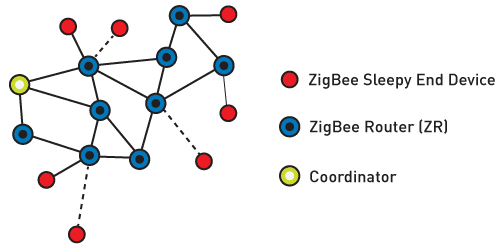
\includegraphics[width=.6\linewidth]{ember-mesh-networking-supported-device}
\caption[Mesh Architecture]{\label{f:ember-mesh-networking-supported-device}Mesh Architecture}
\end{figure}

There are three kinds of nodes :
\begin{itemize}
\item \textbf{A \textit{unique} coordinator} : it is in charge of organizing the network.
\item \textbf{Router} : it is able to propagate the network and is an access point to the network.
\item \textbf{End-node} : it is only able to connect to the network.
\end{itemize}

As we want all the nodes to be the same, we choose to have one coordinator to organize the network and all other nodes are routers. This way, the network can take any configuration possible.

\subsection{Easy Data Packets}

It is very easy to send data packets across the network.

\begin{lstlisting}[frame=single]
#include "firmware_at_api.h"
#include "firmware_api_pack"
//Those two include contains the function
//to easily create tsApiSpec and send them

tsApiSpec apiSpec;
uint8 tmp[sizeof(tsApiSpec)]={0}; 
// Will contain the final result
//For now we put in it a string
sprintf(tmp, "TEST %d", 3); 
// Just a formatted string (like in printf) in tmp
PCK_vApiSpecDataFrame(&apiSpec, 0xec,
                      0x00, tmp, strlen(tmp));
// This function create a DataFrame
uint16 size = i32CopyApiSpec(&apiSpec, tmp); 
//We actually create the array containing 
//the API Frame in tmp
API_bSendToAirPort(UNICAST, 0x0000, tmp, size);
// We send the message to 0x0000, the coordinator
\end{lstlisting}

We begin by writing data into a variable. Then, we create a Data frame with \textbf{PCK\_vApiSpecDataFrame(\&apiSpec, 0xec, 0x00, tmp, strlen(tmp))} which takes as arguments a pointer to the API structure, an identifier for the frame, options for the data frame, the actual data and its size. At that stage, we have a structure which represent our frame.

To make the actual frame (with all bytes at the correct place), we need to use \textbf{i32CopyApiSpec(\&apiSpec, tmp)} which takes a pointer to the structure and an array which will contains the frame. It returns the final size of the frame.

Then the packet can be sent with \textbf{API\_bSendToAirPort(UNICAST, 0x0000, tmp, size)}. We can either choose to BROADCAST or UNICAST a message. Then, we can specify the receiver (0x0000 is the coordinator). Then, we give the frame and its size.

\subsection{A Simple Protocol}

To make the data we send easy to read, we need to specify how data are organize. At the end, a data was composed of three parts :

\begin{itemize}
\item What kind of value the sensor read (temperature, acceleration, humidity,...) on four bytes
\item A time stamp on eight bytes (time in milliseconds, see later)
\item The measurement on four bytes
\end{itemize}

As it has always the same structure, we simplify the sending of data by writing a function in \textbf{src/utils\_meshbee.c} :\textbf{ void send\_frame(char* name, int data)}. The function takes a string of size 4 for the name of the measure and the data read. Then, it sends to the coordinator the formatted frame.

\subsection{AT commands}

It is also possible to communicate with AT commands and to execute a function linked to it, even on an other device. For example, to set the time, we use an AT command which is called from the coordinator to all other nodes. To do so, we need to build a specific frame.

To call a local command, we do :

\begin{lstlisting}[frame=single]
char * aj = "ATMF500";
API_i32AtCmdProc(aj, 7);
\end{lstlisting}

This code set the loop interval to 500ms. We use the function\textbf{ API\_i32AtCmdProc(aj, 7);} which takes the command and its length. It would be also possible to call a remote AT command. Later, we will explain how the server calls these commands.

\subsection{From Zigbee Network to GUI}

Communicating inside the network is quite easy. However, we need a way to show the information that are gathered by the coordinator. To do so, we use a Raspberry Pi which is connected to the coordinator and which controls the network and display measurements.

\subsubsection{Configuring the Raspberry Pi}

We use a Raspberry Pi 3. It is powerful enough to also run a server (see later) and have a Wifi chip integrated. For the OS, we use Raspbian. The first thing we have to do when we is to install the OS. We use a 8Go SD card (less is not enough for the full version of Raspbian). We follow adafruit Raspberry Pi tutorial for example to know how or we search on Google. During the configuration, when we are in raspi-config, we have to remember to activate the serial communication in the advanced parameters.

We need to configure the Serial port to communicate with the MeshBee. We can find the serial port in /dev/ttyS0 on Raspberry Pi 3 or /dev/ttyAMA0 for older versions. The problem is that by default, the raspberry is configured to have a terminal on this port. So we need to remove it. To do so, we open the file /boot/cmdline.txt :

\begin{lstlisting}[frame=single]
sudo nano /boot/cmdline.txt
\end{lstlisting}

and we remove the part with ttyAMA0 or serial0 (console=serial0, 115200). We have something like :

\begin{lstlisting}[frame=single]
dwc_otg.lpm_enable=0 console=tty1 root=/dev/mmcblk0p2
rootfstype=ext4 elevator=deadline rootwait
\end{lstlisting}

(no serial0). What follows is for the Raspberry Pi 3. We need to say that we activate UART. For that, we have to open the file \textbf{/boot/config.txt}

\begin{lstlisting}[frame=single]
sudo nano /boot/config.txt
\end{lstlisting}

and to add the lines

\begin{lstlisting}[frame=single]
enable_uart=1
core_freq=250
\end{lstlisting}

For the version of Raspbian we use, we need to change the core frequency. It may be corrected in future version. We have problems with the communication with the MeshBee. So, by taking an oscilloscope and measuring the baud rate, we measure 72000 instead of  115200.

With the complete version of Raspbian, we do not have to install git and python libraries to manipulate the GPIOs. We clone our Mesh\_Bee repository :

\begin{lstlisting}[frame=single]
git clone https://github.com/Aunsiels/Mesh_Bee.git
\end{lstlisting}

\subsubsection{Connecting the Coordinator with the Raspberry Pi}

Obviously, to communicate with the MeshBee via the serial port, we need to link it to the Raspberry Pi. Here is how the pins are organized on the Raspberry Pi 3.

\begin{figure}[ht]
\centering
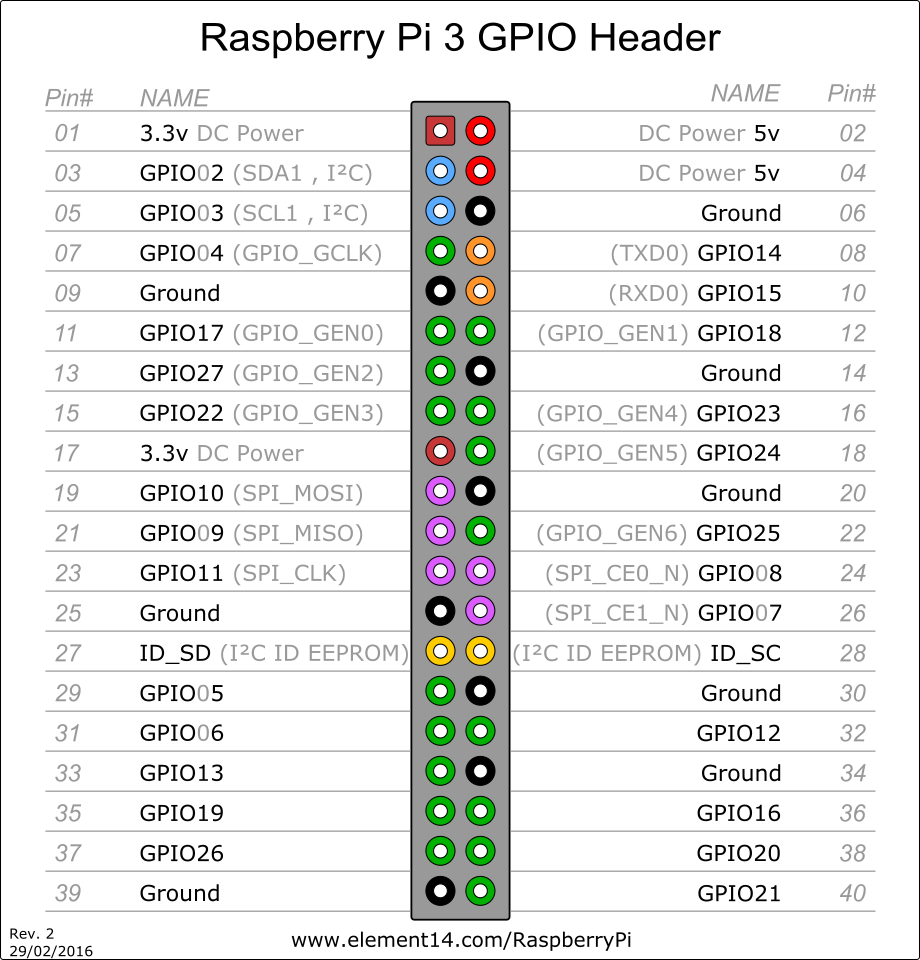
\includegraphics[width=.6\linewidth]{pi3_gpio}
\caption[Pin layout Raspberry Pi]{\label{f:pi3_gpio}Pin layout Raspberry Pi}
\end{figure}

To give power to the MeshBee, we connect the 3.3V pin of the MeshBee to the 3.3V pin of the Raspberry Pi (pin 01). We do the same for Ground (GND) which is on ports 06 or 09 for example. Then, and it is important to do it correctly, to connect the TX1 pin of the MeshBee to the RXD0 pin of the Raspberry Pi (pin 10) and the RX1 pin of the MeshBee to the TXD0 pin of the Raspberry Pi (pin 08). We have something like that :


\begin{figure}[ht]
\centering
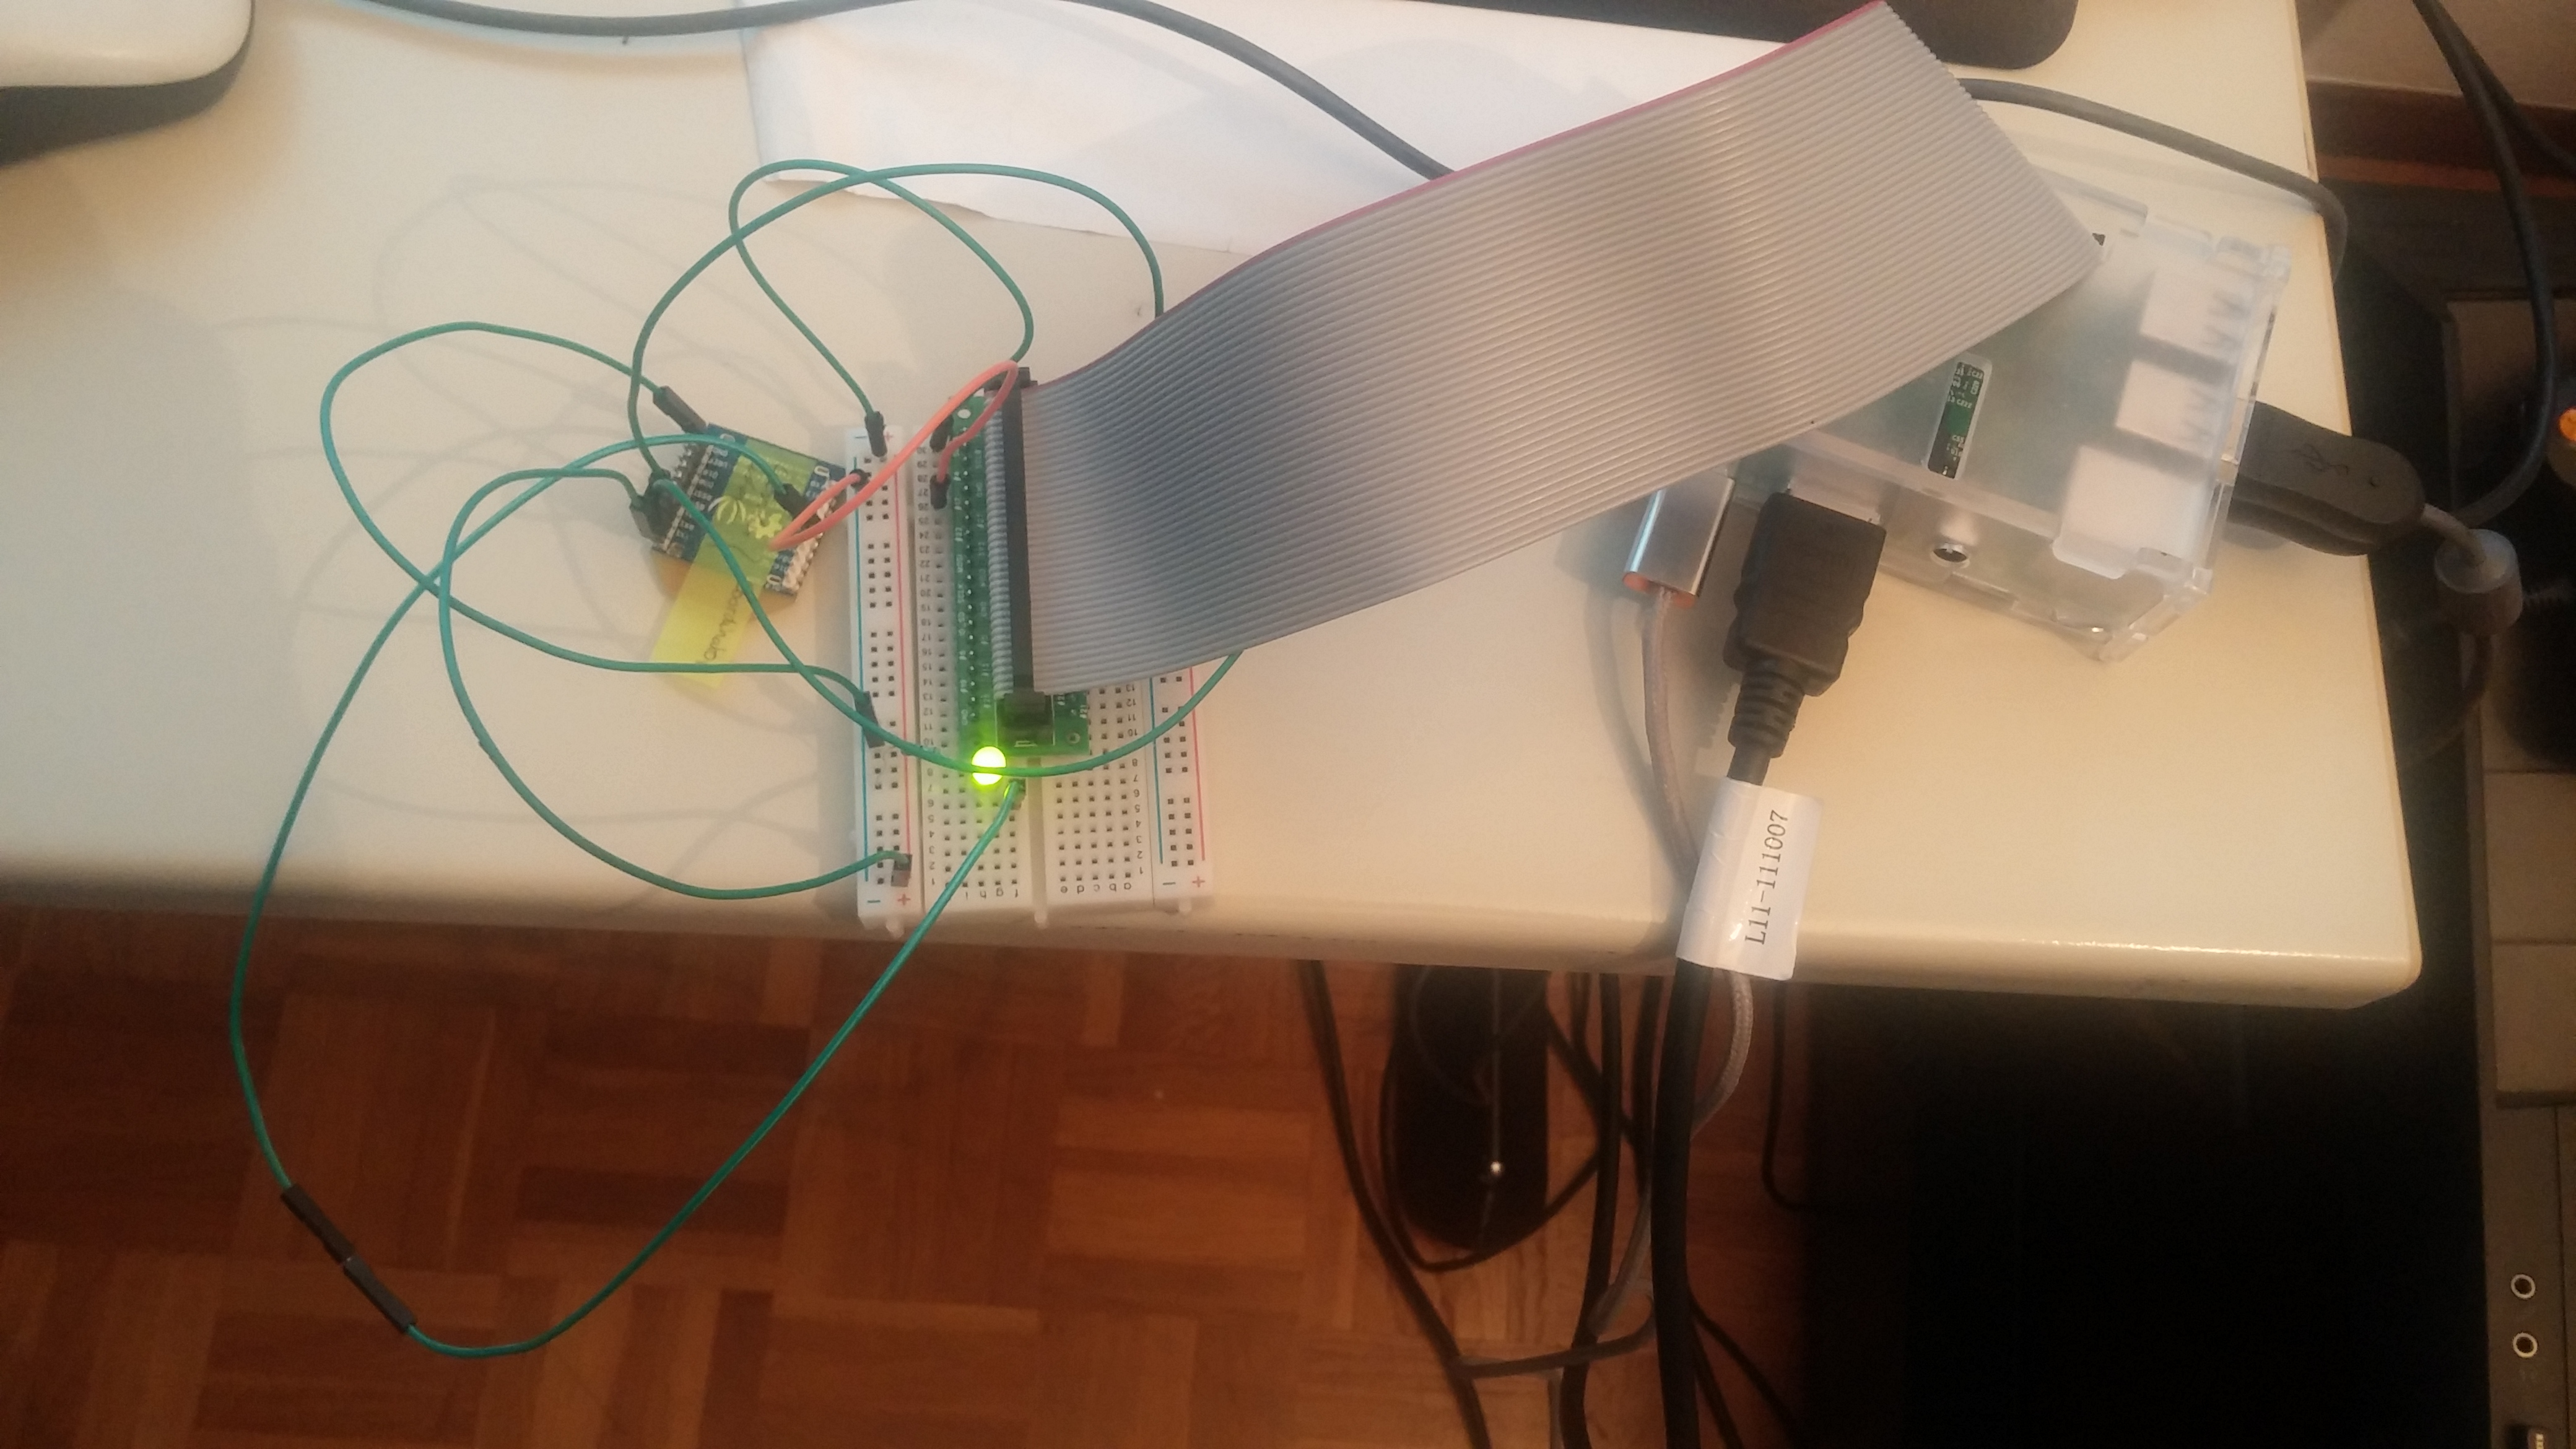
\includegraphics[width=.6\linewidth]{connect_meshbee_rp}
\caption[Photo Connections]{\label{f:connect_meshbee_rp}Photo Connections}
\end{figure}

We add a LED (and a resistor !) connected to the ASSOC pin of the MeshBee to be sure that the MeshBee is connected and working.

We have the MeshBee connected, we try to communicate with it. For that, we use the software cutecom. It is easy to use. We install it :

\begin{lstlisting}[frame=single]
sudo apt-get install cutecom
\end{lstlisting}

Then we open it by typing cutecom in the terminal.

\begin{figure}[ht]
\centering
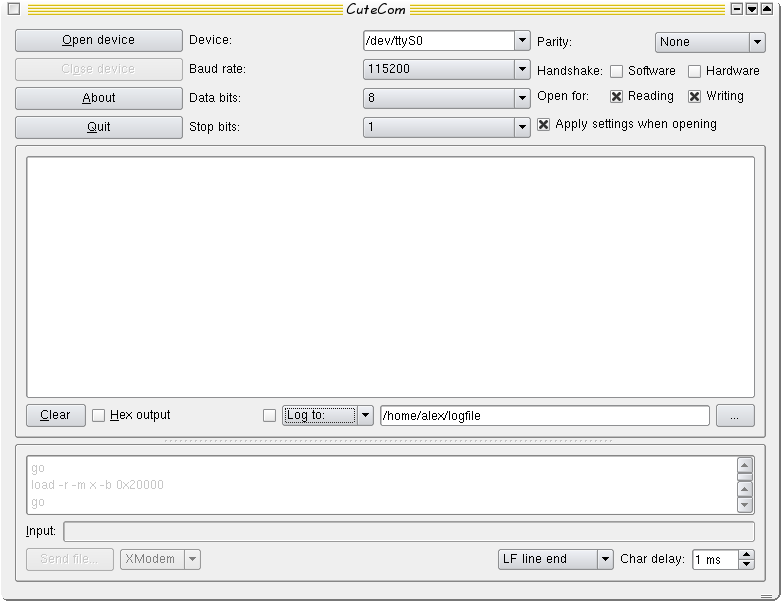
\includegraphics[width=.6\linewidth]{cutecom}
\caption[Cutecom]{\label{f:cutecom}Cutecom}
\end{figure}

Parameters are good when we open it. We just check that the device is /dev/ttyS0 and at the bottom that we have CR line end. We then try to send AT commands for example like we saw above.

\subsubsection{The Python Script}

At that stage, we are sure that we are communicating with the coordinator. We need to automatize the communication and to write a program which can make the connection between the MeshBee network and the server side. The script is \textbf{Mesh\_Bee/rpi\_script.py}. A MeshBee is represented by a class, MeshBee.

The first things we want to do is to be able to change the mode of the coordinator to be sure that we are in the right one. To begin with, we need to initialized the serial connection, when a MeshBee object is created. We use the serial library, which is install be default in the full version of Raspbian. The baud rate is still 115200, and we set the timeout to 1, to be sure we do not get stuck at some point of the program. Then, to facilitate the communication, we use a buffer over the serial. So, to write, we use \textbf{self.meshbee.write} with \textbf{self.meshbee.flush()} (this is very important if we want to actually send). To read, we have self.meshbee.readline or simply \textbf{self.meshbee.read(n)}, where n is the number of byte to read.

To know if we did change the mode, we check what the MeshBee answers. To be sure that there is no old data, we need to empty the buffer before. So, we set the timeout to 0 and read until there is nothing left. We write three functions,\textbf{ to\_at\_mode()}, \textbf{to\_data\_mode()} and \textbf{to\_api\_mode()} to either go to AT, DATA or API mode.

The first experiment we do is only using AT mode and DATA mode. Actually, we use the AT to retrieve information about the network and DATA mode to read the messages. We write two functions for the information : \textbf{print\_information()} which prints information about the current node (it calls ATIF, see above) and \textbf{print\_nodes()} to show the nodes connected to the network. Finally, we have a function to send a message to the entire network, \textbf{write(message)}. Then, we simply read messages in a loop.

The first protocol is very simple : 4 bytes to identify the value read, the id (the mac address) on 8 bytes and then the value read on the rest. At that time, we do not have time synchronization, so no time stamp. However, the mac address is also contained in the DATA frame, we do not have access to it yet.

The problem is that changing the mode can be long (up to a second) and moreover, we lose data by changing the mode. In fact, we want to use the ATLA command to check which nodes are connected to the network (this information can be useful for the user). So, we decide to only use the API mode. Thus, we need to construct and decrypt API frames (see above for API frame structure).

We write a general function to read a frame : \textbf{api\_read\_frame()}. There could be different kind of frames : data frame, topology frame,... We recognize which kind of frame it is and then call the good function to decrypt the payload : \textbf{api\_data\_frame(payload)}, \textbf{api\_topo\_frame(payload)},... While reading the data frame, we retrieve the MAC address, so it is removed from our custom protocol.

So, the new protocol looks like that : 4 bytes to identify the value read, 4 bytes for the time stamp and the rest for the value. We have a time stamp. To share the time, we broadcast an AT command, ATST. This is done thanks to the function \textbf{send\_time()}, which sends the time in second. Finally, we write a function to request the nodes on the network : \textbf{request\_topo()}. We do not have to wait for the result as we did before : each module answers with a frame which is decrypted when received. The mac addresses are stored in an attribute of MeshBee, and they are all sent to the server with \textbf{send\_mac\_addresses()}.

Next we change the time synchronization to milliseconds (see below), the protocol becomes : four bytes to describe the value read, eight bytes for the time stamp and four bytes for the data, which is then totally raw (whereas before it was a string). So, the size is fixed (see above). The \textbf{send\_time()} function then sends time in milliseconds. WARNING : the way bytes are sent is the opposite of the way it is in memory. This is because the endianess is not the same on the MeshBee (Big Endian) and on the computer.

As the server is also on the Raspberry Pi, we just have to send our requests to the localhost domain, port 9000 (see later). Then to send all the mac addresses, we open the URL \textbf{http://localhost:9000/updatesensors?s=} , followed by all MAC addresses.

Finally, we write a main function to call all our functions. This is done in an infinite loop. It just calls \textbf{api\_read\_frame}, and from time to time request to read the network topology and sends a time stamp.

To run the script, we simply type \textbf{python2 rpi\_script.py} in the Mesh\_Bee directory.

\subsubsection{Server Presentation}

We write a HTTP server to retrieve information from the MeshBee network and to display it to the user. The server is written using Play Framework, with Scala. We will not explain how Play Framework works nor how to program in Scala. To run the server, we go to \textbf{Mesh\_Bee/server/bin} and type \textbf{./activator run}. Then we see the port number appear : 9000. The project compiles the first time a page is required.

The configuration of the routes can be found in \textbf{conf/routes}. The HTML files are in \textbf{app/views} and the controllers are in \textbf{app/controllers}. The main controller is \textbf{HomeController.scala}. The code for the real time printing of data thanks to Web sockets is in \textbf{MyWebSocketActor.scala}.

\subsubsection{Record Sensor Data}

The first communication we do with the server is with data directly in the HTTP request. So, to send new measured data to the server, we need to send, to /measuredata :

\begin{lstlisting}[frame=single]
tosend = "http://localhost:9000/measuredata?id=" + id_sensor
tosend = tosend + "&dataType=" + data_type  + "&data=" + data
tosend = tosend + "&time=" + str(time)
\end{lstlisting}
   
The measured data is caught by the measureData function in HomeController.scala. Then, if the data is a special type, we do some computations with the data (for instance, for the temperature, we need to transform the raw data to degrees). Then, we create a Measure object and store it. To keep the user updated, we also send a web socket message to update the chart. Finally, we send a message to confirm we read the measure.

The measured date is first stored in a global variable, \textbf{measures}. We need to take care of concurrent accesses. Later, we will change it by a database access, using MongoDB for instance. However, for development purposes, global variables are easier and easy to clean.

\subsubsection{Real-time Communication}

The real-time communication is done thanks to web sockets. We handle them asynchronously, thanks to actors, in \textbf{app/controllers/MyWebSocketActor.scala}. When we create a web socket, we store it into a map, \textbf{mapping}. So, when a user connects to the page, it creates a web socket. When a new data was received, it is transmitted to all connected users.

\subsubsection{Checking Connected Devices}

When the python wants to tell which devices are connected, it sends the list of all MeshBee as a String. Then, we check if all devices are in the String. Then, the user web page refreshes regularly to keep the printed device list updated. This is done using JavaScript, directly in the HTML page, in app/views.

\subsubsection{Charts}

To print the charts, we used a JavaScript library, Highcharts. The chart was then loaded when the user clicked on a given device.

\begin{figure}[ht]
\centering
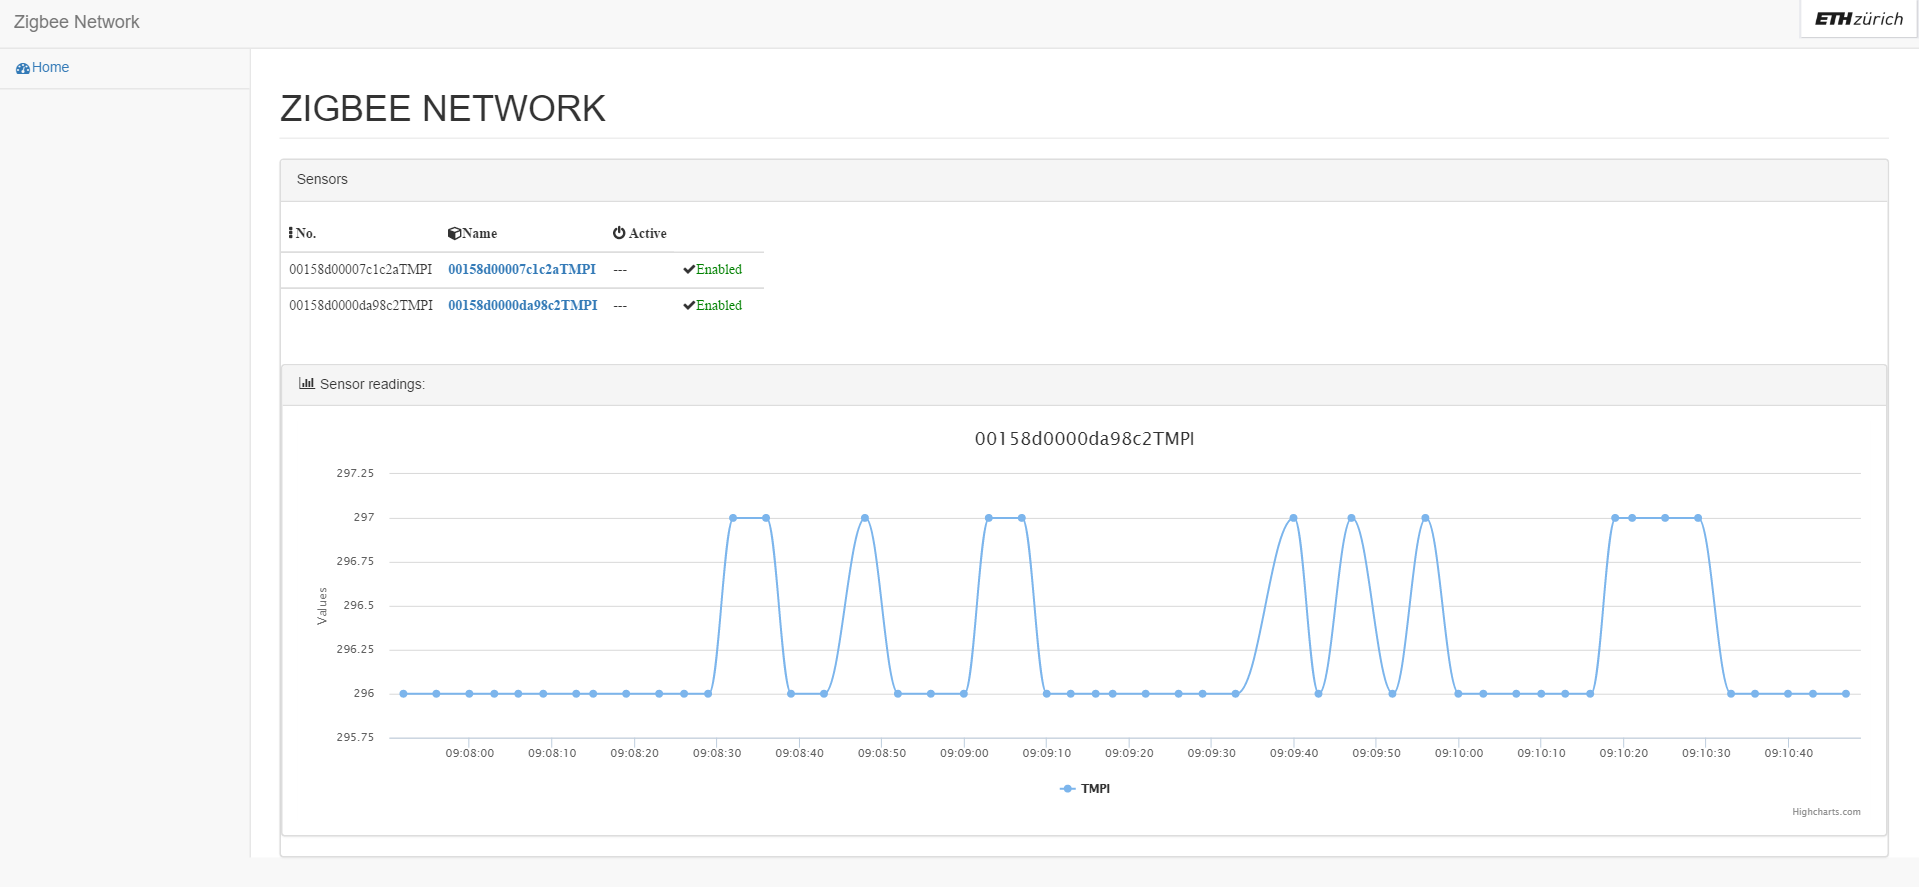
\includegraphics[width=.6\linewidth]{homepage}
\caption[Charts]{\label{f:homepage}Charts}
\end{figure}

\section{Time Synchronization}

\subsection{First Version}

Our first try with time synchronization is to use the given ZCL library (Zigbee Cluster Library). A cluster is something defined in a norm and is a kind of container of data which can be shared in the network. So, it provides us a structure to store data and functions to interact with it. It also updates the time every second thanks to a timer and a task. However, at that time, we do not know that we need to declared everything ourselves in the configuration file. Finally, the library does nothing special as we need to code almost everything. We use the time cluster. The ZCL library can be found in \textbf{Jennic/Components/ZCL}. We have to add the source files of this library to the Makefile.

The first thing we have to do is to give the time to the coordinator. To do so, we create a new AT command we call through the API frame. Creating new AT commands is quite easy. We open the file \textbf{src/firmware\_at\_api.c}. Then, there are two variables : \textbf{atCommands} which is the array containing all AT command which could be called from the AT mode, and atCommands which are commands which can be called from the API mode. We create a new command for API mode, to set the time. So, we add :

\begin{lstlisting}[frame=single]
{"ATST", ATST, NULL, API_setTime_CallBack},
\end{lstlisting}

to atCommandsApiMode. This is a structure of type \textbf{AT\_Command\_ApiMode\_t}, which is defined as follow (in \textbf{include/firmware\_at\_api.h}) :

\begin{lstlisting}[frame=single]
typedef struct
{
    const char  *name;                  
    //AT command name
    uint8       atCmdIndex;             
    //AT command index
    uint16      *configAddr;            
    //config address
    AT_CommandApiMode_Func_t function;  
    //AT commands call back function
}AT_Command_ApiMode_t;
\end{lstlisting}

The name is simply "ATST" (it needs to be four chars). \textbf{atCmdIndex} is a unique number which identifies the command and is generally a constant declared in \textbf{include/firmware\_at\_api.h}, in \textbf{teAtIndex}. ATST has as index 0x80. The configAddr is the address of a variable which will be set to the value given after the AT command (see above to learn more about AT commands). Finally, there is the function which is called for this command. The signature and content are :

\begin{lstlisting}[frame=single]
int API_setTime_CallBack(tsApiSpec *reqApiSpec, tsApiSpec *respApiSpec, uint16 *regAddr)
{
    uint32 time;
    memcpy(&time, reqApiSpec->payload.localAtReq.value, 4);
    vZCL_SetUTCTime(time);

    return OK;
}
\end{lstlisting}

As an argument, we have the received API frame, the frame which will be the answer and the variable which was assigned before and which contains the value of the AT command. We use the memcpy function in order to copy the time stamp in the AT command. Then we use the \textbf{vZCL\_SetUTCTime} function which takes the current time in milliseconds as an argument to set the time of the cluster. To be able to use this function, the time cluster has to be initialized. We do that in the initialization of the node, in \textbf{src/zigbee\_node.}, in the function \textbf{node\_vInitialise}. We use the function \textbf{teZCL\_Status eZCL\_CreateZCL(tsZCL\_Config config);}. This function receives a configuration to initialize the cluster. This configuration contains for instance the callback method for the time cluster, but also other useful information. In the callback method, \textbf{cbZCL\_GeneralCallback in zigbee\_node.c}, we catch some events that can happen. Among them, there can be event to request the ZCL mutex.

It was important to have mutexes when we have interrupts and concurrent accesses. Using mutexes allows us to defined Critical Sections. Critical section is a part of the program which prevents the current task to be pre-empted by an other task from the same mutex group (linked to the same mutex in the configuration file), even by a task of higher priority. To enter a critical section, we use \textbf{OS\_eEnterCriticalSection(name\_mutex);} and to leave it : \textbf{OS\_eExitCriticalSection(name\_mutex);} in vLockZCLMutex and vUnlockZCLMutex (zigbee\_node.c).

Then, we have to call the Event Handler of the time cluster every second. For that, we have to configure a software timer, \textbf{APP\_ZclTimer}, linked to a task, \textbf{APP\_ZCLTask}, which belongs to the ZCL mutex group. In \textbf{APP\_ZCLTask} (in zigbee\_node.c), we call the event handler, vZCL\_EventHandler, which takes a tsZCL\_CallBackEvent as an argument. We put in that structure the kind of event, here E\_ZCL\_CBET\_TIMER.

Then, we have a system to count the time in seconds.

\subsection{Second Version}

Counting in seconds was too restrictive for what we want to do. So we decide to rewrite all the synchronization part to be more flexible and count in milliseconds. The first thing we have to change is to use uint64 instead of uint32. This way, we avoid overflow. In the meanwhile, we also changed the SULI library to also use uint64. The new time synchronization code was written in \textbf{src/time\_sync.c}.

The use is almost the same. There is a function to initialize the variables of the time synchronization : \textbf{void init\_time\_sync(void);}. Then, it is possible to set the low part and the high part of the timestamp with \textbf{void setHighTime(uint32 time);} and \textbf{void setLowTime(uint32 time);}. We have to separate the lowest part and the highest part because for the AT commands, we are only allowed to transmit four bytes of date, half of a uint64. Then, we are able to check whether the time is synchronized or not with int \textbf{timeHasBeenSynchronised(void);} and finally, we can get current time with \textbf{uint64 getTime(void);}. All in all, we replaced all previous functions.

However, we erase the timer part as we do not need to count seconds anymore : we use the SULI \textbf{suli\_millis} function to keep track of the time. We still use mutex as we have concurrent accesses.

As we separate the highest part and the lowest part of the timestamp, we need to do two different AT functions to set the time. ATST is replaced by ATSH (for Set High) and ATSL (for Set Low). The way it works is exactly the same, except that it calls the two functions to set the time.

Once we have done that, the communication protocol changes. A frame is now composed of four bytes to describe the value read, eight bytes for the timestamp and four bytes for the data, which is then totally raw (whereas before it was a string). So, the size is fixed.

\subsection{Correcting the Clocks}

Once we have the framework to synchronize the time, we want to check what is the error of time between all nodes of the network and the server, and how it evolves with time. At first, we are resynchronizing the time every minute, so the error was low, some milliseconds. However, we want to try to only synchronize time once or a limited amount of time and to see how the system evolves. The first experiment we carry out is to compare the time between two MeshBees. Both of them are connected to the Raspberry Pi via wires and Zigbee. The MeshBees synchronize their internal time with the server at the beginning of the experiment. Then, the server sends at regular intervals signals via the wire which trigger an interrupt which sends the current local time. When we plot the time difference between two MeshBees, we observe a drift.

\begin{figure}[ht]
\centering
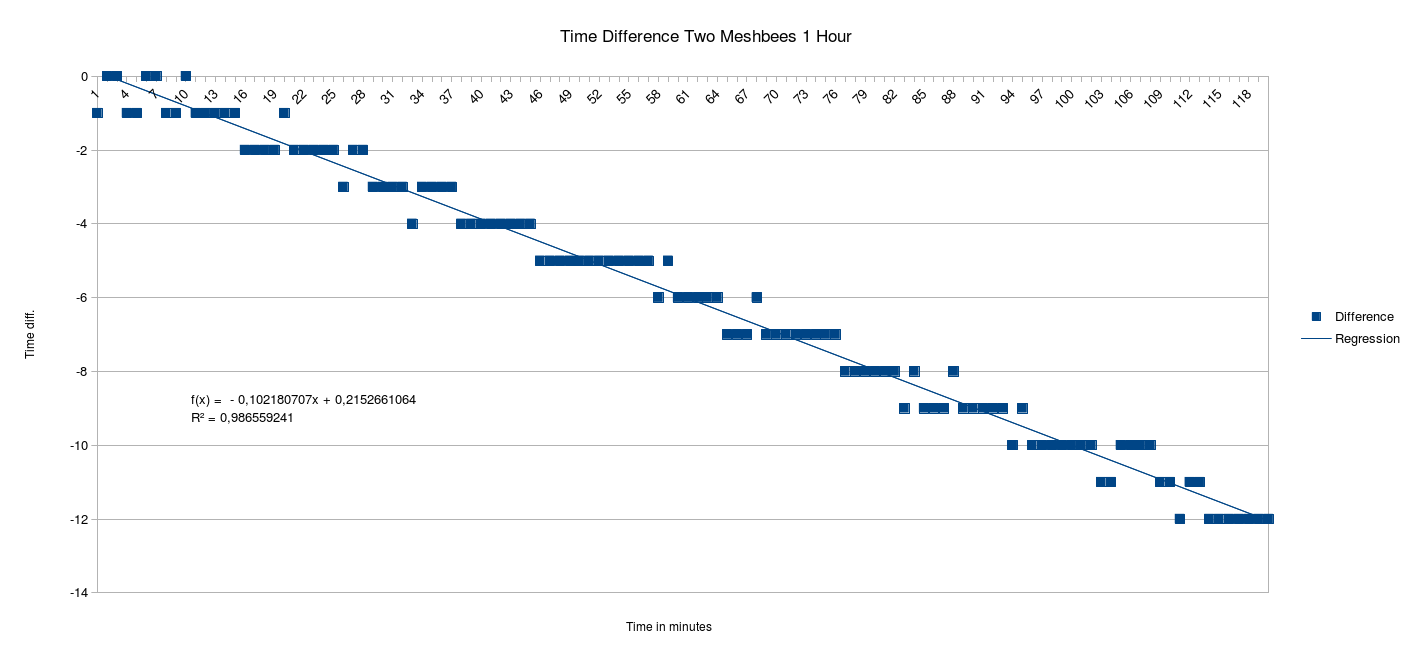
\includegraphics[width=.6\linewidth]{time_sync_1_hour_2meshbees}
\caption[Two meshbees drift]{\label{f:time_sync_1_hour_2meshbees}Two meshbees drift}
\end{figure}

(the time step is 30s) We observe a small drift, of around 0.2 ms per minute. The error can become too big with after a lot of time without synchronization but synchronizing once every 45 minutes give us an error of less than 10ms. Next, we try to see the drift of a MeshBee with the server.

\begin{figure}[ht]
\centering
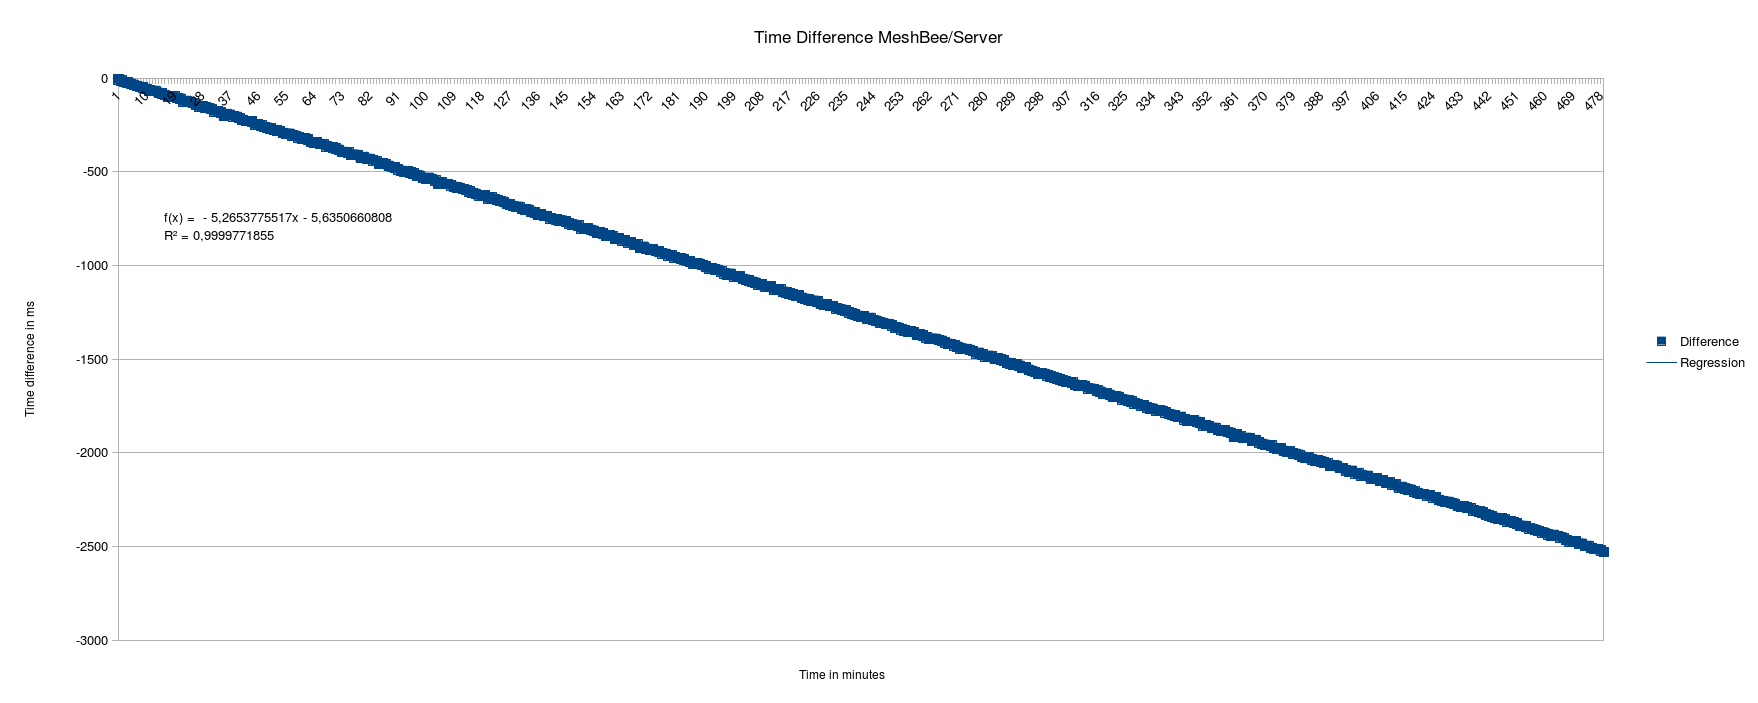
\includegraphics[width=.6\linewidth]{time_sync_8_hours_meshbee_server}
\caption[Meshbee Server Drift]{\label{f:time_sync_8_hours_meshbee_server}MeshBee Server Drift}
\end{figure}

We observe a huge drift, more than 5 ms per minutes. At first, we did not really understand where it was from. However, as it is very linear, we try a simple linear regression to correct it.

\begin{figure}[ht]
\centering
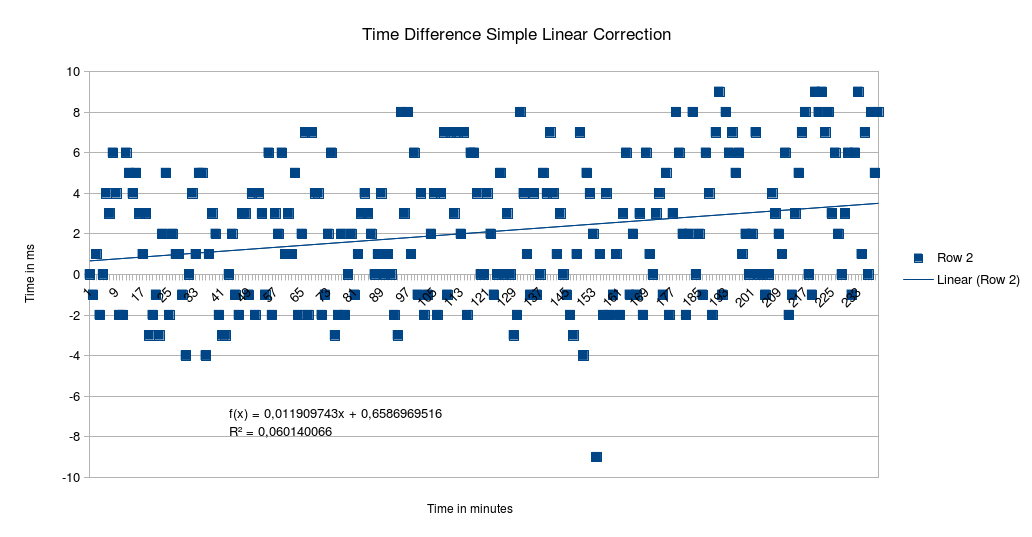
\includegraphics[width=.6\linewidth]{time_difference_simple_regression_server_meshbee}
\caption[Linear Regression Correction]{\label{f:time_difference_simple_regression_server_meshbee}Linear Regression Correction}
\end{figure}

We have some noise due to Zigbee communication but the standard deviation was less than 10 ms. There is almost no drift : 0.012 ms per minutes, even if it is hard to say with the noise. The problem with this approach is that we need to record some samples before being able to correct the read values. To remove this problem, we have to understand where the drift problem is from.

We first think it is because of a stop of the timer due to interrupts, but this is very unlikely because we use a hardware timer. We check that by using an oscilloscope and measuring the clock frequency directly. There seems to be a small problem here. The oscilloscope is not precise enough to be exactly sure, but it seems than the MeshBee clocks are too fast. This hypothesis was not directly considered because an external clock was used and it is supposed to be very precise. However, by reading the documentation, we learn that the clocks have a frequency tolerance of more or less 40ppm (0.004\%). These constraints come from the constraints we have on UART and Zigbee communications. So the 32MHz external clock has a frequency of 32MHz more or less 128kHz, the peripheral frequency (main clock divided by 2) is 16Mhz more or less 64kHz and after the prescaler we use to count time (divided by 16), we have a frequency of 1Mhz more or less 4kHz. So, at the end, in the worst case, we have an error of 4ns every microsecond. So, after one second, we could have an error of 4ms. We measured something smaller but it could be worst.

We explore the possibility to do a calibration of the clock the first time the MeshBee is used with a wired connection. To do so, the MeshBee is connected to the Raspberry Pi with four wires : VCC, GND, a synchronization enable signal (D18) and a clock signal (D1). The clock is generated with a PWM by the Raspberry Pi. A script is used : \textbf{synchronize.py}. Then, the MeshBee catches the interrupt and compare the PWM frequency (which is supposed to be known) and its internal time counter. The correction is computed (in \textbf{utils\_meshbee.c}) and saved permanently in the EEPROM memory by using the PDM library (see in \textbf{time\_sync.c}).

\begin{figure}[ht]
\centering
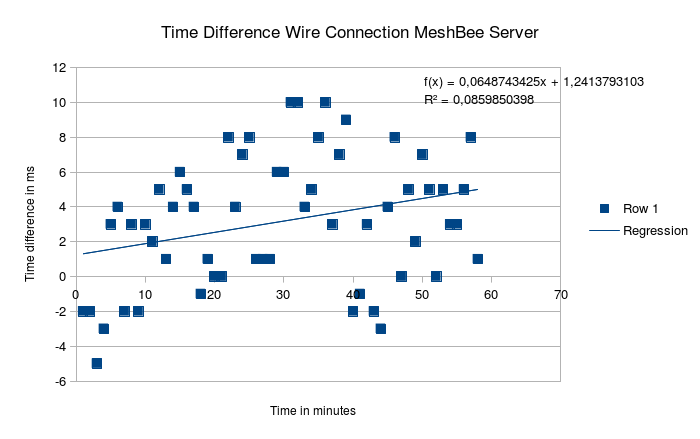
\includegraphics[width=.6\linewidth]{time_sync_wire_correction_meshbee_server}
\caption[Wire Correction]{\label{f:time_sync_wire_correction_meshbee_server}Wire Correction}
\end{figure}

We observe that the drift is reduced and that the noise is still here. There seems to be still a small drift but like for the linear regression correction, it is hard to estimate it on a short time interval. The advantages here are that we do not have to compute coefficients by receiving time steps. We only need the first time stamp to give a good estimate of the future times. However, we cannot correct the bias there can be with only one time stamp. In fact, this bias is due to the noise in Zigbee communication, which makes the first value not centered. However, this bias could be estimated online with similar techniques we used for the linear regression, but we would lose some advantages of the wired method. Another advantage of wire synchronization compared to the linear regression approach is that it does not depend on the size of the network. In big networks the noise will be higher and so linear regression less precise. However, the bias of the wire method will also be higher.

\section{Summary and Contributions}
\label{s:SummaryAndContributions}

Summarize the presented work and demonstrate its contributions to the
research field or institute.



\subsection{Future Work}
\label{s:FutureWork}

Possible ways to extend the work.


% Bibliography
\newpage
\addtocontents{toc}{\vspace{.5\baselineskip}}
\addcontentsline{toc}{section}{\protect\numberline{}{References}}
\bibliography{thesis}


% Appendices (if needed)
\addtocontents{toc}{\vspace{.5\baselineskip}}
\appendix
\section{Extra Stuff}
\label{s:ExtraStuff}

Additional material such as long mathematical derivations.

\section{Examples}
\label{s:Examples}

This appendix provides some additional hints and examples for the
layout and style of the thesis. It is worthwhile to look at the source
file \verb|Examples.tex| for this appendix to understand how it was
created.



\subsection{Tables}

Tables are left justified and the caption appears on top as seen in
Table~\ref{t:Translations}.

\begin{table}[ht]
\caption[Translations]{\label{t:Translations}Translations.}
\begin{tabular}{ll}
\hline
\textbf{English} & \textbf{German}\\
\hline
cell phone       & Handy\\
Diet Coke        & Coca Cola light\\
\hline
\end{tabular}
\end{table}



\subsection{Figures}

Figure~\ref{f:IRISlogo} shows a simple figure with a single picture
and Figure~\ref{f:SubfigureExample} shows a more complex figure
containing subfigures.

\begin{figure}[ht]
\centering

\includegraphics[width=.6\linewidth]{IRISlogo}
\caption[IRIS logo]{\label{f:IRISlogo}IRIS logo.}
\end{figure}

\begin{figure}[ht]
\centering
\subfigure[ETH logo]{
\includegraphics[height=12mm]{ETHlogo}}\quad
\subfigure[IRIS logo]{
\includegraphics[height=12mm]{IRISlogo}}
\caption[Subfigure example]{\label{f:SubfigureExample}Two pictures as
  part of a single figure through the magic of the subfigure package.}
\end{figure}



\subsection{Units}

The SIUnits package provides nice spacing for units as demonstrated in
Table~\ref{t:SIUnits}. Use of the package also makes it easy to change
the style or even the unit text in the future.

\begin{table}[ht]
\caption[Spacing for units]{\label{t:SIUnits}Spacing for units.}
\begin{tabular}{ll}
\hline
\textbf{Output}   & \textbf{Command}\\
\hline
42m               & \verb|42m|\\
\unit{42}{\metre} & \verb|\unit{42}{\metre}|\\
42 m              & \verb|42 m|\\
\hline
\end{tabular}
\end{table}



\subsection{Miscellany}

\begin{description}

\item[Capitalization.] When referring to a named table (such as in the
  previous section), the word \emph{table} is capitalized. The same is
  true for figures, chapters and sections.

\item[Naming of structural elements.] Refer to a \verb|\section| in
  \LaTeX\ as a chapter and call a \verb|\subsection| section. (I don't
  like the way \verb|\chapter|s are rendered in the report document
  class. Hence the suboptimal markup/naming correspondence.)

\item[Bibliography.] Use \verb|bibtex| to make your life easier and to
  produce consistently formatted entries.

\item[Contractions.] Avoid contractions. For instance, use ``do not''
  rather than ``don't.''

\item[Captions.] A brief version of a caption can be provided for the
  list of figures and tables as demonstrated with the caption of
  Figure~\ref{f:SubfigureExample}. The mechanism can also be used to
  get rid of the final period of a caption in the lists.

\end{description}



% Epilogue (optional)
\addtocontents{toc}{\vspace{.5\baselineskip}}
\addcontentsline{toc}{section}{\protect\numberline{}{Epilogue}}
\markright{Epilogue}
\section*{Epilogue}
\label{s:Epilogue}

I hope you found in these pages the starting point of a brilliant idea. Do not hesitate to continue what I started and never sensor yourself. \#blague


\end{document}
